% ---------------------------------------------------------------------------------------------------------------
% TEMPLATE PARA TRABALHO DE CONCLUSÃO DE CURSO
% Universidade Tecnológica Federal do Paraná - UTFPR
% Customização da classe abnTeX2 (http://www.abntex.net.br/) para as normas da UTFPR
%
% Autores: Diego Marczal
% 	       Michael Vornes <https://github.com/mvornes>
% Adaptação (DACOM-CP): Silvio Ricardo Rodrigues Sanches
%
%----------------------------------------------------------------------------------------------------------------
% Codificação: UTF-8
% LaTeX:  abnTeX2          
% ---------------------------------------------------------------------------------------------------------------


% CARREGA CLASSE PERSONALIZADA DA UTFPR--------------------------------------------------------------------------
\documentclass[%twoside,                   % Impressão em frente e verso
    	        oneside,                   % Impressão apenas frente
]{configuracoes/utfpr-abntex2}


% INCLUI ARQUIVOS DE CONFIGURAÇÕES-------------------------------------------------------------------------------
% REFERÊNCIAS------------------------------------------------------------------
\usepackage[%
    alf,
    abnt-emphasize=bf,
    bibjustif,
    recuo=0cm,
    abnt-url-package=url,       % Utiliza o pacote url
    abnt-refinfo=yes,           % Utiliza o estilo bibliográfico abnt-refinfo
    abnt-etal-cite=3,
    abnt-etal-list=3,
    abnt-thesis-year=final
]{abntex2cite}                  % Configura as citações bibliográficas conforme a norma ABNT

% PACOTES----------------------------------------------------------------------
\usepackage[utf8]{inputenc}                                 % Codificação do documento
\usepackage[T1]{fontenc}                                    % Seleção de código de fonte
\usepackage{booktabs}                                       % Réguas horizontais em tabelas
\usepackage{color, colortbl}                                % Controle das cores
\usepackage{float}                                          % Necessário para tabelas/figuras em ambiente multi-colunas
\usepackage{graphicx}                                       % Inclusão de gráficos e figuras
\usepackage{icomma}                                         % Uso de vírgulas em expressões matemáticas
\usepackage{indentfirst}                                    % Indenta o primeiro parágrafo de cada seção
\usepackage{microtype}                                      % Melhora a justificação do documento
\usepackage{multirow, array}                                % Permite tabelas com múltiplas linhas e colunas
\usepackage{subeqnarray}                                    % Permite subnumeração de equações
\usepackage{lastpage}                                       % Para encontrar última página do documento
\usepackage{verbatim}                                       % Permite apresentar texto tal como escrito no documento, ainda que sejam comandos Latex
\usepackage{amsfonts, amssymb, amsmath}                     % Fontes e símbolos matemáticos
\usepackage[algoruled, portuguese]{algorithm2e}             % Permite escrever algoritmos em português
%\usepackage[scaled]{helvet}                                % Usa a fonte Helvetica
\usepackage{times}                                          % Usa a fonte Times
%\usepackage{palatino}                                      % Usa a fonte Palatino
%\usepackage{lmodern}                                       % Usa a fonte Latin Modern
\usepackage[bottom]{footmisc}                               % Mantém as notas de rodapé sempre na mesma posição
\usepackage{ae, aecompl}                                    % Fontes de alta qualidade
\usepackage{latexsym}                                       % Símbolos matemáticos
\usepackage{lscape}                                         % Permite páginas em modo "paisagem"
%\usepackage{picinpar}                                      % Dispor imagens em parágrafos
%\usepackage{scalefnt}                                      % Permite redimensionar tamanho da fonte
%\usepackage{subfig}                                        % Posicionamento de figuras
%\usepackage{upgreek}                                       % Fonte letras gregas

% Redefine a fonte para uma fonte similar a Arial (fonte Helvetica)
\renewcommand*\familydefault{\sfdefault}

% CONFIGURAÇÕES DE APARÊNCIA DO PDF FINAL--------------------------------------
\makeatletter
\hypersetup{%
    portuguese,
    colorlinks=true,   % true: "links" coloridos; false: "links" em caixas de texto
    linkcolor=blue,    % Define cor dos "links" internos
    citecolor=blue,    % Define cor dos "links" para as referências bibliográficas
    filecolor=blue,    % Define cor dos "links" para arquivos
    urlcolor=blue,     % Define a cor dos "hiperlinks"
    breaklinks=true,
    pdftitle={\@title},
    pdfauthor={\@author},
    pdfkeywords={abnt, latex, abntex, abntex2}
}
\makeatother

% ALTERA O ASPECTO DA COR AZUL--------------------------------------------------
\definecolor{blue}{RGB}{41,5,195}

% REDEFINIÇÃO DE LABELS---------------------------------------------------------
\renewcommand{\algorithmautorefname}{Algoritmo}
\def\equationautorefname~#1\null{Equa\c c\~ao~(#1)\null}

% CRIA ÍNDICE REMISSIVO---------------------------------------------------------
\makeindex

% HIFENIZAÇÃO DE PALAVRAS QUE NÃO ESTÃO NO DICIONÁRIO---------------------------
\hyphenation{%
    qua-dros-cha-ve
    Kat-sa-gge-los
}


\graphicspath{{./dados/figuras/}}

% INCLUI ARQUIVOS DO TRABALHO DE CONCLUSÃO DE CURSO (PRÉ-TEXTUAIS, TEXTUAIS, PÓS-TEXTUAIS)-----------------------

% INSERE CAPA E FOLHA DE ROSTO
% CAPA---------------------------------------------------------------------------------------------------

% ORIENTAÇÕES GERAIS-------------------------------------------------------------------------------------
% Caso algum dos campos não se aplique ao seu trabalho, como por exemplo,
% se não houve coorientador, apenas deixe vazio.
% Exemplos: 
% \coorientador{}
% \departamento{}

% DADOS DO TRABALHO--------------------------------------------------------------------------------------
\titulo{Título do Trabalho: Subtítulo do Trabalho}
\titleabstract{Title in English}
\autor{Nome Completo do Autor}
\autorcitacao{SOBRENOME, Nome} % Sobrenome em maiúsculo
\local{Cornélio Procópio}
\data{2018}

% NATUREZA DO TRABALHO-----------------------------------------------------------------------------------
% Opções: 
% - Trabalho de Conclusão de Curso (se for Graduação)
% - Dissertação (se for Mestrado)
% - Tese (se for Doutorado)
% - Projeto de Qualificação (se for Mestrado ou Doutorado)
\projeto{Trabalho de Conclusão de Curso}

% TÍTULO ACADÊMICO---------------------------------------------------------------------------------------
% Opções:
% - Bacharel ou Tecnólogo (Se a natureza for Trabalho de Conclusão de Curso)
% - Mestre (Se a natureza for Dissertação)
% - Doutor (Se a natureza for Tese)
% - Mestre ou Doutor (Se a natureza for Projeto de Qualificação)
\tituloAcademico{...}

% ÁREA DE CONCENTRAÇÃO E LINHA DE PESQUISA---------------------------------------------------------------
% Se a natureza for Trabalho de Conclusão de Curso, deixe ambos os campos vazios
% Se for programa de Pós-graduação, indique a área de concentração e a linha de pesquisa
\areaconcentracao{}
\linhapesquisa{}

% DADOS DA INSTITUIÇÃO-----------------------------------------------------------------------------------
% Se a natureza for Trabalho de Conclusão de Curso, coloque o nome do curso de graduação em "programa"
% Formato para o logo da Instituição: \logoinstituicao{<escala>}{<caminho/nome do arquivo>}
\instituicao{Universidade Tecnológica Federal do Paraná}
\departamento{Departamento Acadêmico de Computação}
\programa{Curso de ...}
\logoinstituicao{0.2}{dados/figuras/logo-instituicao.png} 

% DADOS DOS ORIENTADORES---------------------------------------------------------------------------------
\orientador{Nome do orientador}
%\orientador[Orientadora:]{Nome da orientadora}
\instOrientador{Instituição do orientador}

\coorientador{Nome do coorientador}
%\coorientador[Coorientadora:]{Nome da coorientadora}
\instCoorientador{Instituição do coorientador}

% FOLHA DE ROSTO--------------------------------------------------------------------------------------------------------

% TRABALHO DE CONCLUSÃO DE CURSO
 \preambulo{{\imprimirprojeto} apresentado ao {\imprimirprograma} da {\imprimirinstituicao}, como requisito parcial para a obtenção do título de {\imprimirtituloAcademico}.}

% DISSERTAÇÃO DE MESTRADO
% \preambulo{{\imprimirprojeto} apresentada ao Programa de \mbox{Pós-graduação} da {\imprimirinstituicao}, como requisito parcial para obtenção do título de {\imprimirtituloAcademico}.}

% TESE DE DOUTORADO
% \preambulo{{\imprimirprojeto} apresentada ao Programa de \mbox{Pós-graduação} da {\imprimirinstituicao}, como requisito parcial para a obtenção do título de {\imprimirtituloAcademico}.}

% PROJETO DE QUALIFICAÇÃO DE MESTRADO OU DOUTORADO
%\preambulo{{\imprimirprojeto} apresentado ao Programa de \mbox{Pós-graduação} da {\imprimirinstituicao}, como requisito parcial para a obtenção do título de {\imprimirtituloAcademico}.}

% OBSERVAÇÕES-----------------------------------------------------------------------------------------------------------
% Altere este arquivo APENAS comentando as linhas que não se aplicam ao tipo de trabalho acadêmico desejado.


\begin{document}

\pretextual
\imprimircapa                                               	           % Comando para imprimir Capa
\imprimirfolhaderosto{}                                     		   % Comando para imprimir Folha de rosto
% INSERE ELEMENTOS PRÉ-TEXTUAIS
% DEDICATÓRIA------------------------------------------------------------------

\renewcommand{\dedicatorianame}{DEDICATÓRIA}

\begin{dedicatoria}

Altere este texto inserindo a dedicatória do seu trabalho. 

\end{dedicatoria}
          			   % Dedicatória
% AGRADECIMENTOS---------------------------------------------------------------

\begin{agradecimentos}[AGRADECIMENTOS]

Edite e coloque aqui os agradecimentos às pessoas e/ou instituições que contribuíram para a realização do trabalho.

É obrigatório o agradecimento às instituições de fomento à pesquisa que financiaram total ou parcialmente o trabalho, inclusive no que diz respeito à concessão de bolsas.

\end{agradecimentos}
        			   % Agradecimentos
% EPÍGRAFE---------------------------------------------------------------------

\renewcommand{\epigraphname}{EPÍGRAFE}

\begin{epigrafe}

\textit{Eu denomino meu campo de Gestão do Conhecimento, mas você não pode gerenciar conhecimento. Ninguém pode. O que pode fazer - o que a empresa pode fazer - é gerenciar o ambiente que otimize o conhecimento. (PRUSAK, Laurence, 1997).}

\end{epigrafe}

% OBSERVAÇÕES------------------------------------------------------------------
% Altere o texto para inserir a epígrafe do seu trabalho
              			   % Epígrafe
% RESUMO--------------------------------------------------------------------------------

\begin{resumo}[RESUMO]
\begin{SingleSpacing}

% Não altere esta seção do texto--------------------------------------------------------
\imprimirautorcitacao. \imprimirtitulo. \imprimirdata. \pageref {LastPage} f. \imprimirprojeto\ – \imprimirprograma, \imprimirinstituicao. \imprimirlocal, \imprimirdata.\\
%---------------------------------------------------------------------------------------

O Resumo é um elemento obrigatório em tese, dissertação, monografia e TCC, constituído de uma seqüência de frases concisas e objetivas, fornecendo uma visão rápida e clara do conteúdo do estudo. O texto deverá conter no máximo 500 palavras e ser antecedido
pela referência do estudo. Também, não deve conter citações. O resumo deve ser redigido em parágrafo único, espaçamento simples e seguido das palavras representativas do conteúdo do estudo, isto é, palavras-chave, em número de três a cinco, separadas entre si por ponto e finalizadas também por ponto. Usar o verbo na terceira pessoa do singular, com linguagem impessoal, bem como fazer uso, preferencialmente, da voz ativa. Texto contendo um único parágrafo.\\

\textbf{Palavras-chave}: Palavra. Segunda Palavra. Outra palavra.

\end{SingleSpacing}
\end{resumo}

% OBSERVAÇÕES---------------------------------------------------------------------------
% Altere o texto inserindo o Resumo do seu trabalho.
% Escolha de 3 a 5 palavras ou termos que descrevam bem o seu trabalho 
             			   % Resumo em Português
% ABSTRACT--------------------------------------------------------------------------------

\begin{resumo}[ABSTRACT]
\begin{SingleSpacing}

% Não altere esta seção do texto--------------------------------------------------------
\imprimirautorcitacao. \imprimirtitleabstract. \imprimirdata. \pageref {LastPage} f. \imprimirprojeto\ – \imprimirprograma, \imprimirinstituicao. \imprimirlocal, \imprimirdata.\\
%---------------------------------------------------------------------------------------

Elemento obrigatório em tese, dissertação, monografia e TCC. É a versão do resumo em português para o idioma de divulgação internacional. Deve ser antecedido pela referência do estudo. Deve aparecer em folha distinta do resumo em língua portuguesa e seguido das palavras representativas do conteúdo do estudo, isto é, das palavras-chave. Sugere-se a elaboração do resumo (Abstract) e das palavras-chave (Keywords) em inglês; para resumos em outras línguas, que não o inglês, consultar o departamento / curso de origem.\\

\textbf{Keywords}: Word. Second Word. Another word.

\end{SingleSpacing}
\end{resumo}

% OBSERVAÇÕES---------------------------------------------------------------------------
% Altere o texto inserindo o Abstract do seu trabalho.
% Escolha de 3 a 5 palavras ou termos que descrevam bem o seu trabalho 
             		           % Resumo em Inglês
% Lista de Figuras----------------------------------------------------------------

\pdfbookmark[0]{\listfigurename}{lof}
\listoffigures*
\cleardoublepage

% OBSERVAÇÕES---------------------------------------------------------------------
% Este arquivo não precisa de ser alterado, pois a lista é gerada automaticamente.
   % Lista de Figuras
% LISTA DE QUADROS----------------------------------------------------------------

\renewcommand{\listofquadrosname}{LISTA DE QUADROS}

\pdfbookmark[0]{\listofquadrosname}{loq}
\listofquadros*
\cleardoublepage

% OBSERVAÇÕES---------------------------------------------------------------------
% Este arquivo não necessita de ser editado. A lista é gerada automaticamente.
   % Lista de Quadros
% LISTA DE TABELAS-------------------------------------------------------------

\pdfbookmark[0]{\listtablename}{lot}
\listoftables*
\cleardoublepage

% OBSERVAÇÕES-------------------------------------------------------------------
% Este arquivo não precisa ser alterado, pois a lista é gerada automaticamente.
         		   % Lista de Tabelas
% LISTA DE ABREVIATURAS E SIGLAS----------------------------------------------------------

\begin{siglas}
    \item[ABNT] Associação Brasileira de Normas Técnicas
    \item[DECOM] Departamento de Computação
\end{siglas}

% OBSERVAÇÕES-----------------------------------------------------------------------------
% Altere a lista acima para definir os acrônimos e siglas utilizados neste trabalho
          		   % Lista de Abreviaturas e Siglas
% LISTA DE SÍMBOLOS------------------------------------------------------------

\begin{simbolos}
    \item[$ \Gamma $] Letra grega Gama
    \item[$ \lambda $] Comprimento de onda
    \item[$ \in $] Pertence
\end{simbolos}

% OBSERVAÇÕES-------------------------------------------------------------------
% Altere a lista acima para definir os símbolos utilizados no trabalho
        		   % Lista de Símbolos
% LISTA DE ALGORITMOS----------------------------------------------------------

\newcommand{\algoritmoname}{Algoritmo}
\renewcommand{\listalgorithmcfname}{LISTA DE ALGORITMOS}

\floatname{algocf}{\algoritmoname}
\newlistof{listofalgoritmos}{loa}{\listalgoritmoname}
\newlistentry{algocf}{loa}{0}

\counterwithout{algocf}{chapter}
\renewcommand{\cftalgocfname}{\algoritmoname\space}
\renewcommand*{\cftalgocfaftersnum}{\hfill--\hfill}

\pdfbookmark[0]{\listalgorithmcfname}{loa}
\listofalgorithms
\cleardoublepage

% OBSERVAÇÕES------------------------------------------------------------------
% Este arquivo não precisa ser alterado, pois a lista é gerada automaticamente.
   % Lista de Algoritmos
% SUMÁRIO----------------------------------------------------------------------

\renewcommand{\contentsname}{SUMÁRIO}

\pdfbookmark[0]{\contentsname}{toc}
\tableofcontents*
\cleardoublepage

% OBSERVAÇÕES-------------------------------------------------------------------
% Este arquivo não precisa ser alterado, pois o sumário é gerado automaticamente.
               			   % Sumário

\textual
% INSERE ELEMENTOS TEXTUAIS
% INTRODUÇÃO-------------------------------------------------------------------

\chapter{INTRODUÇÃO}
\label{chap:introducao}

Edite e coloque aqui o seu texto de introdução.

A Introdução é a parte inicial do texto, na qual devem constar o tema e a delimitação do assunto tratado, objetivos da pesquisa e outros elementos necessários para situar o tema do trabalho, tais como: justificativa, procedimentos metodológicos (classificação inicial), embasamento teórico (principais bases sintetizadas) e estrutura do trabalho, tratados de forma sucinta. Recursos utilizados e cronograma são incluídos quando necessário. Salienta-se que os procedimentos metodológicos e o embasamento teórico são tratados, posteriormente, em capítulos próprios e com a profundidade necessária ao trabalho de pesquisa.

\section{LEIA ESTA SEÇÃO ANTES DE COMEÇAR}
\label{sec:antesleiame}

Este documento é um \emph{template} \LaTeX{} que foi concebido, primariamente, para ser utilizado na elaboração de Trabalho de Conclusão de Curs em conformidade com as normas da Universidade Tecnológica Federal do Paraná.

Para a produção deste \emph{template} foi necessário adaptar o arquivo {\ttfamily abntex2.cls}. Assim, foi produzido o arquivo {\ttfamily utfpr-abntex2.cls} que define o \verb|documentclass| específico para a UTFPR.

Antes de começar a escrever o seu trabalho acadêmico utilizando este \emph{template}, é importante saber que há dois arquivos que você precisará editar para que a capa e a folha de rosto de seu trabalho sejam geradas automaticamente.
São eles os arquivos {\ttfamily capa.tex} e {\ttfamily folha-rosto.tex}, ambos no diretório  {\ttfamily /elementos-pre-textuais}.
No arquivo {\ttfamily capa.tex} deverá ser informado nome do autor, título do trabalho, natureza do trabalho, nome do orientador e outras informações necessárias.
No arquivo {\ttfamily folha-rosto.tex}, que contém o texto padrão estabelecendo que este documento é um requisito parcial para a obtenção do título pretendido, será necessário apenas comentar as linhas que não se aplicam ao tipo de trabalho acadêmico.

A compilação para gerar um arquivo no formato pdf, incluindo corretamente as referências bibliográficas, deve ser realizada utilizando o comando \verb|makefile|, disponível na mesma pasta onde está o arquivo principal \verb|utfpr-tcc.tex|. Caso seja alterado o nome do arquivo \verb|utfpr-tcc.tex|, deverá ser alterado no arquivo \verb|makefile| também.

\section{ORGANIZAÇÃO DO TRABALHO}
\label{sec:organizacaoTrabalho}

Normalmente ao final da introdução é apresentada, em um ou dois parágrafos curtos, a organização do restante do trabalho acadêmico.
Deve-se dizer o quê será apresentado em cada um dos demais capítulos.
                		           % Introdução
% REVISÃO DE LITERATURA--------------------------------------------------------

\chapter{REVISÃO DE LITERATURA}
\label{chap:fundamentacaoTeorica}

É uma boa prática iniciar cada novo capítulo com um breve texto introdutório (tipicamente, dois ou três parágrafos) que deve deixar claro o quê será discutido no capítulo, bem como a organização do capítulo.
Também servirá ao propósito de "amarrar"{} o conteúdo deste capítulo com o conteúdo do capítulo imediatamente anterior.
         % Revisão de Literatura
% METODOLOGIA------------------------------------------------------------------

\chapter{METODOLOGIA}
\label{chap:metodologia}
Cada capítulo deve conter uma pequena introdução (tipicamente, um ou dois parágrafos) que deve deixar claro o objetivo e o que será discutido no capítulo, bem como a organização do capítulo.

\section{DELINEAMENTO DA PESQUISA}
\label{sec:titSecDelPesq}

Inserir seu texto aqui...

\section{COLETA E TRATAMENTO DE DADOS}
\label{sec:titSecColDad}

Inserir seu texto aqui...
                   % Metodologia
% REQUISITOS------------------------------------------------------------------

\chapter{ANÁLISE E PROJETO DO SISTEMA}
\label{chap:analise}
Neste capítulo serão exibidos os Requisitos Funcionais e Não Funcionais, bem como a Especificação dos Requisitos Funcionais, o Diagrama de Casos de Uso Geral, o Diagrama de Classes e o Diagrama Entidade-Relacionamento.

\subsection{Requisitos Funcionais}
\label{sec:titSecReqFunc}

Os requisitos funcionais são artefatos gerados pela especificação de requisitos, que é o processo de escrever os requisitos de usuário e de sistema em um documento de requisitos. Preferencialmente, os requisitos de usuário e sistema devem ser claros, inequívocos, de fácil compreensão, completos e consistentes. Porém, na prática, é difícil que isso ocorra, visto que os envolvidos no processo veem os requisitos de formas diferentes, e em grande parte das vezes, nota-se conflitos e inconsistências relacionadas à esses requisitos \cite{Sommerville10}.

No presente projeto os requisitos foram obtidos com base na planilha de cálculo de correção e equilíbrio do solo, fornecida pelo cliente, utilizando a técnica de etnografia, que consiste em uma técnica de observação que pode ser usada na elicitação e análise de requisitos. O etnógrafo imerge no ambiente dos usuários e observa os hábitos de seu trabalho diário. Os requisitos de software podem ser deduzidos a partir dessas observações \cite{Sommerville10}.

\begin{landscape}
\begin{longtable}{|p{1.5cm}|p{5cm}|p{9cm}|p{2.5cm}|}
    \hline
    ID    & REQUISITO                                                                        & DESCRIÇÃO                                                                                                                                                                                                                                                                                               & PRIORIDADE \\\hline
    \endfirsthead
    %
    \hline
    ID    & REQUISITO                                                                        & DESCRIÇÃO                                                                                                                                                                                                                                                                                               & PRIORIDADE \\\hline
    \endhead
    %
    RF001 & Gerenciar informações da propriedade.                                            & O sistema deve permitir ao usuário cadastrar, remover, alterar ou listar informações do solo de um produtor.                                                                                                                                                                                            & Essencial  \\\hline
    RF002 & Gerenciar nutrientes do solo.                                                    & O sistema deve permitir ao usuário inserir, remover, alterar ou listar os nutrientes coletados na análise do solo.                                                                                                                                                                                      & Essencial  \\\hline
    RF003 & Exibir valores ideais.                                                           & O sistema deve exibir os valores ideais de cada teor inserido de acordo com a textura do solo.                                                                                                                                                                                                          & Importante \\\hline
    RF004 & Exibir valores dos nutrientes após correções.                                    & O sistema deve exibir os valores dos nutrientes inseridos após as correções.                                                                                                                                                                                                                            & Importante \\\hline
    RF005 & Gerenciar matéria orgânica.                                                      & O sistema deve permitir ao usuário inserir, remover, alterar ou listar o teor da matéria orgânica (M.O.) do solo.                                                                                                                                                                                       & Essencial  \\\hline
    RF006 & Exibir teor ideal da M.O.                                                        & O sistema deve exibir o teor ideal de matéria orgânica (M.O.).                                                                                                                                                                                                                                          & Importante \\\hline
    RF007 & Gerenciar dados relacionados à correção/recuperação  de Fósforo.                 & O sistema deve permitir ao usuário cadastrar, remover,  alterar ou listar valores ligados ao Fósforo, tais como teor a ser atingido, fonte a ser utilizada e eficiência.                                                                                                                                & Essencial  \\\hline
    RF008 & Exibir valores a serem aplicados no processo de correção/recuperação de Fósforo. & O sistema deve informar ao usuário a quantidade de Fósforo à ser aplicada assim como o seu custo.                                                                                                                                                                                                       & Importante \\\hline
    RF009 & Gerenciar valor/ton. (R\$) no processo relacionado às fontes de Fósforo.         & O sistema deve possibilitar ao usuário inserir, remover, alterar ou listar valores relacionados às fontes: superfosfato simples, superfosfato triplo, MAP, DAP, Yoorin, Fosfato Arad, Fosfato Gafsa, Fosfato Daoui, Fosfato  Patos Minas, Escória de Thomas, ácido Fosfórico e multifosfato magnesiano. & Essencial  \\\hline
    RF010 & Gerenciar dados relacionados à correção/recuperação do Potássio.                 & O sistema deve possibilitar ao usuário inserir, remover,  alterar ou listar dados relacionados à participação do Potássio na CTC assim como a fonte de Potássio a ser usada.                                                                                                                            & Essencial  \\\hline
    RF011 & Exibir valores relacionados à correção/recuperação do Potássio.                  & O sistema deve informar ao usuário dados à respeito do Potássio tais como: participação atual na CTC do solo,  participação do Potássio na CTC após correção, quantidade e custo a ser aplicada e sua participação ideal na CTC.                                                                        & Importante \\\hline
    RF012 & Gerenciar valor/ton. (R\$) no processo relacionado às fontes de Potássio.        & O sistema deve permitir ao usuário cadastrar, excluir, alterar ou listar valores como: cloreto de Potássio, Sulfato de Potássio e Sulfato de Potássio/Magnésio.                                                                                                                                         & Essencial  \\\hline
    RF013 & Cadastrar dados para a correção do cálcio e magnésio no solo                     & O sistema deve permitir o usuário informar dados acerca da correção do cálcio no solo.                                                                                                                                                                                                                  & Essencial \\\hline
    RF014 & Alterar dados para a correção do cálcio e magnésio no solo                       & O sistema deve permitir o usuário alterar os dados sobre a correção do solo.                                                                                                                                                                                                                            & Desejável  \\\hline
    RF015 & Exibir o teor de cálcio atualmente no solo                                       & O sistema deve apresentar ao usuário, o percentual de Cálcio na CTC atual (antes das correções)                                                                                                                                                                                                         & Essencial  \\\hline
    RF016 & Exibir o teor de cálcio ideal no solo                                            & O sistema deve apresentar ao usuário, o intervalo percentual de Cálcio ideal na CTC.                                                                                                                                                                                                                    & Importante  \\\hline
    RF017 & Calcular o percentual de cálcio ideal no solo                                    & O sistema deve apresentar ao usuário, o percentual ideal de Cálcio na CTC.                                                                                                                                                                                                                              & Importante  \\\hline
    RF018 & Exibir teor de magnésio atualmente no solo                                       & O sistema deve apresentar ao usuário o percentual de Magnésio atual na CTC.                                                                                                                                                                                                                             & Importante  \\\hline
    RF019 & Exibir o percentual ideal de magnésio no solo                                    & O sistema deve apresentar ao usuário o percentual de Magnésio ideal na CTC.                                                                                                                                                                                                                             & Importante  \\\hline
    RF020 & Exibir o valor do magnésio no solo após as correções                             & O sistema deve apresentar ao usuário o percentual de Magnésio na CTC após as correções.                                                                                                                                                                                                                 & Importante  \\\hline
    RF021 & Calcular o teor de magnésio no solo após as correções                            & O sistema deve calcular o percentual de Magnésio na CTC após as correções.                                                                                                                                                                                                                              & Importante  \\\hline
    RF022 & Exibir a quantidade de corretivo de cálcio e magnésio a ser aplicada no solo.    & O sistema deve exibir a quantidade a ser aplicada, em toneladas por hectare, do corretivo informado.                                                                                                                                                                                                    & Importante  \\\hline
    RF023 & Calcular a quantidade de corretivo a ser aplicada no solo.                       & O sistema deve calcular a quantidade a ser aplicada, em toneladas por hectare, do corretivo informado.                                                                                                                                                                                                  & Importante  \\\hline
    RF024 & Exibir a quantidade de enxofre que o corretivo fornecerá à terra                 & O sistema deve exibir o valor, em quilogramas por hectare, da quantidade de enxofre que o corretivo fornecerá.                                                                                                                                                                                          & Desejável  \\\hline
    RF025 & Exibir a quantidade de enxofre necessária                                        & O sistema deve exibir a quantidade suficiente, em quilogramas por hectare, da quantidade de enxofre necessária.                                                                                                                                                                                         & Desejável  \\\hline
    RF026 & Calcular e exibir o valor de V\% atual, ideal e após as correções                & O sistema deve calcular e exibir os valores de V\% atual, ideal e após as correções.                                                                                                                                                                                                                    & Importante  \\\hline
    \caption{Tabela de Requisitos Funcionais}
    \label{rf:tabela}
\end{longtable}
\end{landscape}

\clearpage

\begin{quadro}[!htb]
    \begin{tabular}{|p{3cm}|p{11cm}|}
        \hline
        \textbf{RS300} & \textbf{Cadastrar dados para a correção do cálcio e magnésio no solo} \\
        \hline
        Sumário        & O sistema deve permitir o usuário informar dados acerca da correção do cálcio no solo.                  \\
        \hline
        Pré-condições  & O usuário deve estar logado no sitema                  \\
        \hline
        Atores         & Usuário                  \\
        \hline
        Descrição      &
        \begin{itemize}
            \item Informa o percentual de cálcio desejado na CTC
            \item Seleciona qual fonte de cálcio será utilizada na correção
            \item Informa o custo médio em R\$/ha do corretivo
            \item Informa o percentual de PRNT do corretivo
            \item Informa o teor de CaO do corretivo
        \end{itemize}                 \\
        \hline
        Alternativas   &
        \begin{itemize}
            \item Caso o usuário não saiba o teor de CaO, será utilizado o valor médio do corretivo
        \end{itemize}                 \\
        \hline
        Exceção        &
        \begin{itemize}
            \item Caso o usuário informe um valor percental fora do intervalo de 0 a 100, não poderá proseguir com o preenchimento de outros campos.
            \item Caso o usuário informa um corretivo que não exista, uma mensagem de erro deverá ser exibida.
        \end{itemize}                   \\
        \hline
    \end{tabular}
\end{quadro}

\begin{quadro}[!htb]
    \begin{tabular}{|p{3cm}|p{11cm}|}
        \hline
        \textbf{RS301} & \textbf{Alterar dados para a correção do cálcio e magnésio no solo} \\
        \hline
        Sumário        & O sistema deve permitir o usuário alterar os dados sobre a correção do solo.                  \\
        \hline
        Pré-condições  & \begin{itemize}
            \item O usuário deve estar logado
            \item O usuário deverá acessar uma ??análise?? já existente 
        \end{itemize}                 \\
        \hline
        Atores         & Usuário                  \\
        \hline
        Descrição      &
        \begin{itemize}
            \item Informa o percentual de cálcio desejado na CTC
            \item Seleciona qual fonte de cálcio será utilizada na correção
            \item Informa o custo médio em R\$/ha do corretivo
            \item Informa o percentual de PRNT do corretivo
            \item Informa o teor de CaO do corretivo
        \end{itemize}                 \\
        \hline
        Alternativas   &
        \begin{itemize}
            \item Caso o usuário não saiba o teor de CaO, será utilizado o valor médio do corretivo
        \end{itemize}                 \\
        \hline
        Exceção        &
        \begin{itemize}
            \item Caso o usuário informe um valor percental fora do intervalo de 0 a 100, não poderá proseguir com o preenchimento de outros campos.
            \item Caso o usuário informe um corretivo que não exista, uma mensagem de erro deverá ser exibida.
        \end{itemize}                   \\
        \hline
    \end{tabular}
\end{quadro}

\begin{quadro}[!htb]
    \begin{tabular}{|p{3cm}|p{11cm}|}
        \hline
        \textbf{RS302} & \textbf{Alterar dados para a correção do cálcio e magnésio no solo} \\
        \hline
        Sumário        & O sistema deve permitir o usuário alterar os dados sobre a correção do solo.                  \\
        \hline
        Pré-condições  & \begin{itemize}
            \item O usuário deve estar logado
            \item O usuário deverá acessar uma ??análise?? já existente 
        \end{itemize}                 \\
        \hline
        Atores         & Usuário                  \\
        \hline
        Descrição      &
        \begin{itemize}
            \item Informa o percentual de cálcio desejado na CTC
            \item Seleciona qual fonte de cálcio será utilizada na correção
            \item Informa o custo médio em R\$/ha do corretivo
            \item Informa o percentual de PRNT do corretivo
            \item Informa o teor de CaO do corretivo
        \end{itemize}                 \\
        \hline
        Alternativas   &
        \begin{itemize}
            \item Caso o usuário não saiba o teor de CaO, será utilizado o valor médio do corretivo
        \end{itemize}                 \\
        \hline
        Exceção        &
        \begin{itemize}
            \item Caso o usuário informe um valor percental fora do intervalo de 0 a 100, não poderá proseguir com o preenchimento de outros campos.
            \item Caso o usuário informe um corretivo que não exista, uma mensagem de erro deverá ser exibida.
        \end{itemize}                   \\
        \hline
    \end{tabular}
\end{quadro}

\begin{quadro}[!htb]
    \begin{tabular}{|p{3cm}|p{11cm}|}
        \hline
        \textbf{RS303} & \textbf{Alterar dados para a correção do cálcio e magnésio no solo} \\
        \hline
        Sumário        & O sistema deve permitir o usuário alterar os dados sobre a correção do solo.                  \\
        \hline
        Pré-condições  & \begin{itemize}
            \item O usuário deve estar logado
            \item O usuário deverá acessar uma ??análise?? já existente 
        \end{itemize}                 \\
        \hline
        Atores         & Usuário                  \\
        \hline
        Descrição      &
        \begin{itemize}
            \item Informa o percentual de cálcio desejado na CTC
            \item Seleciona qual fonte de cálcio será utilizada na correção
            \item Informa o custo médio em R\$/ha do corretivo
            \item Informa o percentual de PRNT do corretivo
            \item Informa o teor de CaO do corretivo
        \end{itemize}                 \\
        \hline
        Alternativas   &
        \begin{itemize}
            \item Caso o usuário não saiba o teor de CaO, será utilizado o valor médio do corretivo
        \end{itemize}                 \\
        \hline
        Exceção        &
        \begin{itemize}
            \item Caso o usuário informe um valor percental fora do intervalo de 0 a 100, não poderá proseguir com o preenchimento de outros campos.
            \item Caso o usuário informe um corretivo que não exista, uma mensagem de erro deverá ser exibida.
        \end{itemize}                   \\
        \hline
    \end{tabular}
\end{quadro}

\begin{quadro}[!htb]
    \begin{tabular}{|p{3cm}|p{11cm}|}
        \hline
        \textbf{RS304} & \textbf{Alterar dados para a correção do cálcio e magnésio no solo} \\
        \hline
        Sumário        & O sistema deve permitir o usuário alterar os dados sobre a correção do solo.                  \\
        \hline
        Pré-condições  & \begin{itemize}
            \item O usuário deve estar logado
            \item O usuário deverá acessar uma ??análise?? já existente 
        \end{itemize}                 \\
        \hline
        Atores         & Usuário                  \\
        \hline
        Descrição      &
        \begin{itemize}
            \item Informa o percentual de cálcio desejado na CTC
            \item Seleciona qual fonte de cálcio será utilizada na correção
            \item Informa o custo médio em R\$/ha do corretivo
            \item Informa o percentual de PRNT do corretivo
            \item Informa o teor de CaO do corretivo
        \end{itemize}                 \\
        \hline
        Alternativas   &
        \begin{itemize}
            \item Caso o usuário não saiba o teor de CaO, será utilizado o valor médio do corretivo
        \end{itemize}                 \\
        \hline
        Exceção        &
        \begin{itemize}
            \item Caso o usuário informe um valor percental fora do intervalo de 0 a 100, não poderá proseguir com o preenchimento de outros campos.
            \item Caso o usuário informe um corretivo que não exista, uma mensagem de erro deverá ser exibida.
        \end{itemize}                   \\
        \hline
    \end{tabular}
\end{quadro}

\begin{quadro}[!htb]
    \begin{tabular}{|p{3cm}|p{11cm}|}
        \hline
        \textbf{RS305} & \textbf{Alterar dados para a correção do cálcio e magnésio no solo} \\
        \hline
        Sumário        & O sistema deve permitir o usuário alterar os dados sobre a correção do solo.                  \\
        \hline
        Pré-condições  & \begin{itemize}
            \item O usuário deve estar logado
            \item O usuário deverá acessar uma ??análise?? já existente 
        \end{itemize}                 \\
        \hline
        Atores         & Usuário                  \\
        \hline
        Descrição      &
        \begin{itemize}
            \item Informa o percentual de cálcio desejado na CTC
            \item Seleciona qual fonte de cálcio será utilizada na correção
            \item Informa o custo médio em R\$/ha do corretivo
            \item Informa o percentual de PRNT do corretivo
            \item Informa o teor de CaO do corretivo
        \end{itemize}                 \\
        \hline
        Alternativas   &
        \begin{itemize}
            \item Caso o usuário não saiba o teor de CaO, será utilizado o valor médio do corretivo
        \end{itemize}                 \\
        \hline
        Exceção        &
        \begin{itemize}
            \item Caso o usuário informe um valor percental fora do intervalo de 0 a 100, não poderá proseguir com o preenchimento de outros campos.
            \item Caso o usuário informe um corretivo que não exista, uma mensagem de erro deverá ser exibida.
        \end{itemize}                   \\
        \hline
    \end{tabular}
\end{quadro}

\begin{quadro}[!htb]
    \begin{tabular}{|p{3cm}|p{11cm}|}
        \hline
        \textbf{RS306} & \textbf{Alterar dados para a correção do cálcio e magnésio no solo} \\
        \hline
        Sumário        & O sistema deve permitir o usuário alterar os dados sobre a correção do solo.                  \\
        \hline
        Pré-condições  & \begin{itemize}
            \item O usuário deve estar logado
            \item O usuário deverá acessar uma ??análise?? já existente 
        \end{itemize}                 \\
        \hline
        Atores         & Usuário                  \\
        \hline
        Descrição      &
        \begin{itemize}
            \item Informa o percentual de cálcio desejado na CTC
            \item Seleciona qual fonte de cálcio será utilizada na correção
            \item Informa o custo médio em R\$/ha do corretivo
            \item Informa o percentual de PRNT do corretivo
            \item Informa o teor de CaO do corretivo
        \end{itemize}                 \\
        \hline
        Alternativas   &
        \begin{itemize}
            \item Caso o usuário não saiba o teor de CaO, será utilizado o valor médio do corretivo
        \end{itemize}                 \\
        \hline
        Exceção        &
        \begin{itemize}
            \item Caso o usuário informe um valor percental fora do intervalo de 0 a 100, não poderá proseguir com o preenchimento de outros campos.
            \item Caso o usuário informe um corretivo que não exista, uma mensagem de erro deverá ser exibida.
        \end{itemize}                   \\
        \hline
    \end{tabular}
\end{quadro}

\begin{quadro}[!htb]
    \begin{tabular}{|p{3cm}|p{11cm}|}
        \hline
        \textbf{RS307} & \textbf{Alterar dados para a correção do cálcio e magnésio no solo} \\
        \hline
        Sumário        & O sistema deve permitir o usuário alterar os dados sobre a correção do solo.                  \\
        \hline
        Pré-condições  & \begin{itemize}
            \item O usuário deve estar logado
            \item O usuário deverá acessar uma ??análise?? já existente 
        \end{itemize}                 \\
        \hline
        Atores         & Usuário                  \\
        \hline
        Descrição      &
        \begin{itemize}
            \item Informa o percentual de cálcio desejado na CTC
            \item Seleciona qual fonte de cálcio será utilizada na correção
            \item Informa o custo médio em R\$/ha do corretivo
            \item Informa o percentual de PRNT do corretivo
            \item Informa o teor de CaO do corretivo
        \end{itemize}                 \\
        \hline
        Alternativas   &
        \begin{itemize}
            \item Caso o usuário não saiba o teor de CaO, será utilizado o valor médio do corretivo
        \end{itemize}                 \\
        \hline
        Exceção        &
        \begin{itemize}
            \item Caso o usuário informe um valor percental fora do intervalo de 0 a 100, não poderá proseguir com o preenchimento de outros campos.
            \item Caso o usuário informe um corretivo que não exista, uma mensagem de erro deverá ser exibida.
        \end{itemize}                   \\
        \hline
    \end{tabular}
\end{quadro}

\begin{quadro}[!htb]
    \begin{tabular}{|p{3cm}|p{11cm}|}
        \hline
        \textbf{RS308} & \textbf{Alterar dados para a correção do cálcio e magnésio no solo} \\
        \hline
        Sumário        & O sistema deve permitir o usuário alterar os dados sobre a correção do solo.                  \\
        \hline
        Pré-condições  & \begin{itemize}
            \item O usuário deve estar logado
            \item O usuário deverá acessar uma ??análise?? já existente 
        \end{itemize}                 \\
        \hline
        Atores         & Usuário                  \\
        \hline
        Descrição      &
        \begin{itemize}
            \item Informa o percentual de cálcio desejado na CTC
            \item Seleciona qual fonte de cálcio será utilizada na correção
            \item Informa o custo médio em R\$/ha do corretivo
            \item Informa o percentual de PRNT do corretivo
            \item Informa o teor de CaO do corretivo
        \end{itemize}                 \\
        \hline
        Alternativas   &
        \begin{itemize}
            \item Caso o usuário não saiba o teor de CaO, será utilizado o valor médio do corretivo
        \end{itemize}                 \\
        \hline
        Exceção        &
        \begin{itemize}
            \item Caso o usuário informe um valor percental fora do intervalo de 0 a 100, não poderá proseguir com o preenchimento de outros campos.
            \item Caso o usuário informe um corretivo que não exista, uma mensagem de erro deverá ser exibida.
        \end{itemize}                   \\
        \hline
    \end{tabular}
\end{quadro}

\begin{quadro}[!htb]
    \begin{tabular}{|p{3cm}|p{11cm}|}
        \hline
        \textbf{RS309} & \textbf{Alterar dados para a correção do cálcio e magnésio no solo} \\
        \hline
        Sumário        & O sistema deve permitir o usuário alterar os dados sobre a correção do solo.                  \\
        \hline
        Pré-condições  & \begin{itemize}
            \item O usuário deve estar logado
            \item O usuário deverá acessar uma ??análise?? já existente 
        \end{itemize}                 \\
        \hline
        Atores         & Usuário                  \\
        \hline
        Descrição      &
        \begin{itemize}
            \item Informa o percentual de cálcio desejado na CTC
            \item Seleciona qual fonte de cálcio será utilizada na correção
            \item Informa o custo médio em R\$/ha do corretivo
            \item Informa o percentual de PRNT do corretivo
            \item Informa o teor de CaO do corretivo
        \end{itemize}                 \\
        \hline
        Alternativas   &
        \begin{itemize}
            \item Caso o usuário não saiba o teor de CaO, será utilizado o valor médio do corretivo
        \end{itemize}                 \\
        \hline
        Exceção        &
        \begin{itemize}
            \item Caso o usuário informe um valor percental fora do intervalo de 0 a 100, não poderá proseguir com o preenchimento de outros campos.
            \item Caso o usuário informe um corretivo que não exista, uma mensagem de erro deverá ser exibida.
        \end{itemize}                   \\
        \hline
    \end{tabular}
\end{quadro}

\begin{quadro}[!htb]
    \begin{tabular}{|p{3cm}|p{11cm}|}
        \hline
        \textbf{RS310} & \textbf{Alterar dados para a correção do cálcio e magnésio no solo} \\
        \hline
        Sumário        & O sistema deve permitir o usuário alterar os dados sobre a correção do solo.                  \\
        \hline
        Pré-condições  & \begin{itemize}
            \item O usuário deve estar logado
            \item O usuário deverá acessar uma ??análise?? já existente 
        \end{itemize}                 \\
        \hline
        Atores         & Usuário                  \\
        \hline
        Descrição      &
        \begin{itemize}
            \item Informa o percentual de cálcio desejado na CTC
            \item Seleciona qual fonte de cálcio será utilizada na correção
            \item Informa o custo médio em R\$/ha do corretivo
            \item Informa o percentual de PRNT do corretivo
            \item Informa o teor de CaO do corretivo
        \end{itemize}                 \\
        \hline
        Alternativas   &
        \begin{itemize}
            \item Caso o usuário não saiba o teor de CaO, será utilizado o valor médio do corretivo
        \end{itemize}                 \\
        \hline
        Exceção        &
        \begin{itemize}
            \item Caso o usuário informe um valor percental fora do intervalo de 0 a 100, não poderá proseguir com o preenchimento de outros campos.
            \item Caso o usuário informe um corretivo que não exista, uma mensagem de erro deverá ser exibida.
        \end{itemize}                   \\
        \hline
    \end{tabular}
\end{quadro}

\begin{quadro}[!htb]
    \begin{tabular}{|p{3cm}|p{11cm}|}
        \hline
        \textbf{RS311} & \textbf{Informar o valor por tonelada do corretivo} \\
        \hline
        Sumário        & O sistema deve permitir o usuário alterar os dados sobre a correção do solo.                  \\
        \hline
        Pré-condições  & \begin{itemize}
            \item O usuário deve estar logado
            \item O usuário deverá acessar uma ??análise?? já existente 
        \end{itemize}                 \\
        \hline
        Atores         & Usuário                  \\
        \hline
        Descrição      &
        \begin{itemize}
            \item Informa o percentual de cálcio desejado na CTC
            \item Seleciona qual fonte de cálcio será utilizada na correção
            \item Informa o custo médio em R\$/ha do corretivo
            \item Informa o percentual de PRNT do corretivo
            \item Informa o teor de CaO do corretivo
        \end{itemize}                 \\
        \hline
        Alternativas   &
        \begin{itemize}
            \item Caso o usuário não saiba o teor de CaO, será utilizado o valor médio do corretivo
        \end{itemize}                 \\
        \hline
        Exceção        &
        \begin{itemize}
            \item Caso o usuário informe um valor percental fora do intervalo de 0 a 100, não poderá proseguir com o preenchimento de outros campos.
            \item Caso o usuário informe um corretivo que não exista, uma mensagem de erro deverá ser exibida.
        \end{itemize}                   \\
        \hline
    \end{tabular}
\end{quadro}

\begin{quadro}[!htb]
    \begin{tabular}{|p{3cm}|p{11cm}|}
        \hline
        \textbf{RS312} & \textbf{Calcular e exibir a quantidade de corretivo a ser aplicada no solo.} \\
        \hline
        Sumário        & O sistema deve calcular a quantidade a ser aplicada, em toneladas por hectare, do corretivo informado.                  \\
        \hline
        Pré-condições  & \begin{itemize}
            \item O usuário deve estar logado
            \item O usuário deverá acessar uma ??análise?? já existente 
        \end{itemize}                 \\
        \hline
        Atores         & Usuário                  \\
        \hline
        Descrição      &
        \begin{itemize}
            \item Informa o percentual de cálcio desejado na CTC
            \item Seleciona qual fonte de cálcio será utilizada na correção
            \item Informa o custo médio em R\$/ha do corretivo
            \item Informa o percentual de PRNT do corretivo
            \item Informa o teor de CaO do corretivo
        \end{itemize}                 \\
        \hline
        Alternativas   &
        \begin{itemize}
            \item Caso o usuário não saiba o teor de CaO, será utilizado o valor médio do corretivo
        \end{itemize}                 \\
        \hline
        Exceção        &
        \begin{itemize}
            \item Caso o usuário informe um valor percental fora do intervalo de 0 a 100, não poderá proseguir com o preenchimento de outros campos.
            \item Caso o usuário informe um corretivo que não exista, uma mensagem de erro deverá ser exibida.
        \end{itemize}                   \\
        \hline
    \end{tabular}
\end{quadro}

\begin{quadro}[!htb]
    \begin{tabular}{|p{3cm}|p{11cm}|}
        \hline
        \textbf{RS313} & \textbf{Exibir o custo do corretivo em reais por hectare} \\
        \hline
        Sumário        & O sistema deve calcular e exibir o custo em reais (R\$ por hectare do corretivo informado.                  \\
        \hline
        Pré-condições  & \begin{itemize}
            \item O usuário deve estar logado
            \item O usuário deverá acessar uma ??análise?? já existente 
        \end{itemize}                 \\
        \hline
        Atores         & Usuário                  \\
        \hline
        Descrição      &
        \begin{itemize}
            \item Informa o percentual de cálcio desejado na CTC
            \item Seleciona qual fonte de cálcio será utilizada na correção
            \item Informa o custo médio em R\$/ha do corretivo
            \item Informa o percentual de PRNT do corretivo
            \item Informa o teor de CaO do corretivo
        \end{itemize}                 \\
        \hline
        Alternativas   &
        \begin{itemize}
            \item Caso o usuário não saiba o teor de CaO, será utilizado o valor médio do corretivo
        \end{itemize}                 \\
        \hline
        Exceção        &
        \begin{itemize}
            \item Caso o usuário informe um valor percental fora do intervalo de 0 a 100, não poderá proseguir com o preenchimento de outros campos.
            \item Caso o usuário informe um corretivo que não exista, uma mensagem de erro deverá ser exibida.
        \end{itemize}                   \\
        \hline
    \end{tabular}
\end{quadro}

\begin{quadro}[!htb]
    \begin{tabular}{|p{3cm}|p{11cm}|}
        \hline
        \textbf{RS314} & \textbf{Exibir a quantidade de enxofre que o corretivo fornecerá à terra} \\
        \hline
        Sumário        & O sistema deve exibir o valor, em quilogramas por hectare, da quantidade de enxofre que o corretivo fornecerá.                  \\
        \hline
        Pré-condições  & \begin{itemize}
            \item O usuário deve estar logado
            \item O usuário deverá acessar uma ??análise?? já existente 
        \end{itemize}                 \\
        \hline
        Atores         & Usuário                  \\
        \hline
        Descrição      &
        \begin{itemize}
            \item Informa o percentual de cálcio desejado na CTC
            \item Seleciona qual fonte de cálcio será utilizada na correção
            \item Informa o custo médio em R\$/ha do corretivo
            \item Informa o percentual de PRNT do corretivo
            \item Informa o teor de CaO do corretivo
        \end{itemize}                 \\
        \hline
        Alternativas   &
        \begin{itemize}
            \item Caso o usuário não saiba o teor de CaO, será utilizado o valor médio do corretivo
        \end{itemize}                 \\
        \hline
        Exceção        &
        \begin{itemize}
            \item Caso o usuário informe um valor percental fora do intervalo de 0 a 100, não poderá proseguir com o preenchimento de outros campos.
            \item Caso o usuário informe um corretivo que não exista, uma mensagem de erro deverá ser exibida.
        \end{itemize}                   \\
        \hline
    \end{tabular}
\end{quadro}

\begin{quadro}[!htb]
    \begin{tabular}{|p{3cm}|p{11cm}|}
        \hline
        \textbf{RS315} & \textbf{Exibir a quantidade de enxofre necessária} \\
        \hline
        Sumário        & O sistema deve exibir a quantidade suficiente, em quilogramas por hectare, da quantidade de enxofre necessária.                  \\
        \hline
        Pré-condições  & \begin{itemize}
            \item O usuário deve estar logado
            \item O usuário deverá acessar uma ??análise?? já existente 
        \end{itemize}                 \\
        \hline
        Atores         & Usuário                  \\
        \hline
        Descrição      &
        \begin{itemize}
            \item Informa o percentual de cálcio desejado na CTC
            \item Seleciona qual fonte de cálcio será utilizada na correção
            \item Informa o custo médio em R\$/ha do corretivo
            \item Informa o percentual de PRNT do corretivo
            \item Informa o teor de CaO do corretivo
        \end{itemize}                 \\
        \hline
        Alternativas   &
        \begin{itemize}
            \item Caso o usuário não saiba o teor de CaO, será utilizado o valor médio do corretivo
        \end{itemize}                 \\
        \hline
        Exceção        &
        \begin{itemize}
            \item Caso o usuário informe um valor percental fora do intervalo de 0 a 100, não poderá proseguir com o preenchimento de outros campos.
            \item Caso o usuário informe um corretivo que não exista, uma mensagem de erro deverá ser exibida.
        \end{itemize}                   \\
        \hline
    \end{tabular}
\end{quadro}

\begin{quadro}[!htb]
    \begin{tabular}{|p{3cm}|p{11cm}|}
        \hline
        \textbf{RS316} & \textbf{Calcular e exibir o valor de V\% atual, ideal e após as correções} \\
        \hline
        Sumário        & O sistema deve calcular e exibir os valores de V\% atual, ideal e após as correções.                  \\
        \hline
        Pré-condições  & \begin{itemize}
            \item O usuário deve estar logado
            \item A etapa de preenchimento dos dados da propriedade deverá estar preenchida 
            \item A etapa de preenchimento da análise do solo deverá estar preenchida 
            \item A etapa de preenchimento da matéria orgânica deverá está preenchida 
            \item A etapa de preenchimento da correção do fósforo deverá estar preenchida 
            \item A etapa de preenchimento da correção do postássio deverá estar preenchida 
            \item A etapa de preenchimento da correção do cálcio e magnésio' deverá estar preenchida 
        \end{itemize}                 \\
        \hline
        Atores         & Usuário                  \\
        \hline
        Descrição      &
        \begin{itemize}
            \item O sistema realiza o cálculo do V\% atual
            \item O sistema exibe o resultado do cálculo do V\% atual
            \item O sistema realiza o cálculo do V\% após as correções
            \item O sistema exibe o resultado do cálculo do V\% após as correções
            \item O sistema realiza o cálculo do V\% ideal
            \item O sistema exibe o resultado do cálculo do V\% ideal
        \end{itemize}                 \\
        \hline
        Alternativas   &
        \begin{itemize}
            \item Sem alternativas
        \end{itemize}                 \\
        \hline
        Exceção        &
        \begin{itemize}
            \item Sem exceções
        \end{itemize}                   \\
        \hline
    \end{tabular}
\end{quadro}
\clearpage

\subsection{Requisitos Não Funcionais}
\label{sec:titSecReqNaoFunc}

Os requisitos não funcionais representam restrições que vão além das funcionalidades de um sistema. Eles podem estar relacionados à alguma necessidade emergente do sistema como o tempo de resposta ou o espaço de armazenamento. Esses requisitos, normalmente, são aplicado ao sistema todo, ao invés de uma funcionalidade ou serviço específico \cite{pressman2016engenharia}.

Na \autoref{rnf:tabela} encontram-se os requisitos funcionais levantados para essa aplicação.

\begin{landscape}
\begin{longtable}{|p{1.5cm}|p{4.5cm}|p{10cm}|p{3cm}|}
    \hline
    ID     & REQUISITO                                                    & DESCRIÇÃO                                                                                                                         & CATEGORIA        \\\hline
    \endfirsthead
    %
    \multicolumn{4}{c}%
    {{\bfseries Continuação da tabela \thetable\ da página anterior}}                                                                                                                                                            \\\hline
    ID     & REQUISITO                                                    & DESCRIÇÃO                                                                                                                         & CATEGORIA        \\\hline
    \endhead
    %
    RNF001 & O sistema deve ser responsivo.                               & O sistema deve se adaptar em diferentes tamanhos de tela com proporção 16:9.                                                      & Usabilidade      \\\hline
    RNF002 & Validação no front-end.                                       & Todos os formulários, exceto os de autenticação, devem ser validados no navegador sem que haja o recarregamento da página.         & Usabilidade      \\\hline
    RNF003 & Não permitir o acesso de visitantes às páginas internas.     & O sistema deve validar a permissão do usuário ao tentar acessar uma página restrita.                                              & Segurança        \\\hline
    RNF004 & Backup automático.                                           & O sistema deverá realizar um backup automaticamente todos os dias às 4:00, de acordo com o horário de Brasília.                   & Segurança        \\\hline
    RNF005 & O código escrito deverá ser entendível.                      & Um profissional com 1 ano de experiência com PHP deverá conseguir criar um CRUD na API em até 8 horas de leitura.                 & Manutenibilidade \\\hline
    RNF006 & Criptografia de dados sensíveis.                             & O sistema deve criptografar as senhas dos usuários.                                                                               & Segurança        \\\hline
    RNF007 & Bloqueio de acesso externo.                                  & O servidor de banco de dados só poderá ser acessado pela rede local do servidor.                                                  & Segurança        \\\hline
    RNF008 & Inicar nova correção em até 3 cliques.                       & O sistema deve permitir o usuário autenticado, a partir de qualquer tela, acessar o formulário de nova correção em até 3 cliques. & Usabilidade      \\\hline
    RNF009 & O sistema deve ser acessível por meio de um nome de domínio. & O usuário poderá acessar o sistema por meio de um nome de domínio.                                                                & Usabilidade      \\\hline
    \caption{Tabela de Requisitos Não Funcionais}
    \label{rnf:tabela}
\end{longtable}
\end{landscape}

\clearpage

\subsection{Casos de Uso}
\label{sec:titSecCasoUso}

Segundo \citeonline{guedes2018uml}, o diagrama de casos de uso "apresenta uma linguagem simples e de fácil compreensão para que os usuários possam ter uma ideia geral de como o sistema irá se comportar". São extremamente úteis para expor aos interessados no projeto, as funcionalidades que compõem a aplicação.

\begin{figure}[H]
    \centering
    \caption{Diagrama de Caso de Uso Geral}
    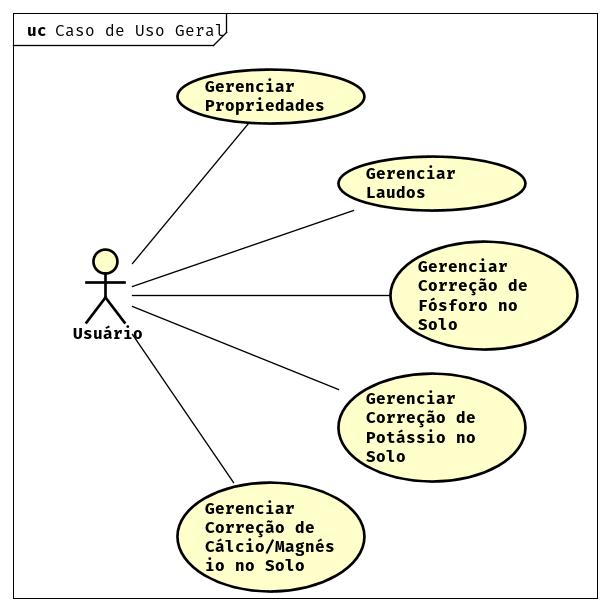
\includegraphics[width=13cm]{dados/figuras/casouso.jpg}
    \label{fig:diagramaCasoUso}
    \fonte{Autoria própria}
\end{figure}

Os casos de uso estão intimamente relacionados aos requisitos funcionais enumerados na \autoref{rf:tabela} e que serão comentados nas subseções abaixo.

\subsubsection{Caso de Uso - Gerenciar propriedades}
\label{sec:titSecCasoUsoPropriedades}

O Caso de Uso "Gerenciar propriedades" está relacionado ao requisito funcional RF001. Um propriedade representa uma área pertencente à um agricultor, como um sítio ou fazenda. Cada propriedade possui uma ou várias partições ou talhões, que será analisada, sendo assim, de suma importância para o funcionamento da aplicação. Como um produtor pode ter várias áreas analisadas em uma propriedades, faz-se necessário a criação de uma entidade no sistema.

\subsubsection{Caso de Uso - Gerenciar laudos}
\label{sec:titSecCasoUsoLaudos}

O caso de uso "Gerenciar laudos" referencia os RF02 a RF06. O laudo técnico do solo representa os indicadores de nutrientes do solo de um determinado talhão. Um talhão pode ser analisado diversas vezes. Por isso é importante que este laudo seja gerenciável como uma entidade na aplicação.

\subsubsection{Caso de Uso - Gerenciar correção de fósforo no solo}
\label{sec:titSecCasoUsoFosforo}

O caso de uso "Gerenciar correção de fósforo no solo" referencia os RF07 a RF09. As variáveis de correção do solo são: fonte de corretivo, eficiência, custo por tonelada. As fontes de corretivo possuem um valor padrão, que o usuário poderá editar no momento da realização do cálculo pois um determinado corretivo pode ser vendido com o mesmo nome mas ter propriedades diferentes. Por isso é necessário tornar gerenciável.

\subsubsection{Caso de Uso - Gerenciar correção de potássio no solo}
\label{sec:titSecCasoUsoPotassio}

O caso de uso "Gerenciar correção de potássio no solo" referencia os RF10 a RF12. Caso a saturação de bases fique além do ideal, é possível alterar o percentual desejado de potássio na CTC. Também deve ser possível o usuário alterar o valor em R\$/ton da fonte de potássio.

\subsubsection{Caso de Uso - Gerenciar correção do cálcio e magnésio no solo}
\label{sec:titSecCasoUsoCalcioMagnesio}

O caso de uso "Gerenciar correção do cálcio e magnésio no solo" referencia os RF13 a RF25. Caso a saturação de bases fique além do necessário, o usuário do sistema poderá corrigir o percentual de cálcio desejado na CTC. Além disso, também deve ser possível o usuário alterar o valor padrão do PRNT do corretivo, bem como o valor em R\$/ton.
\clearpage

\section{Diagrama de Classes}
\label{sec:titSecDiagClasse}

O Diagrama de Classes, segundo \cite{guedes2018uml}, define a estrutura das classes utilizadas pelo sistema, determinando os atributos e métodos que cada classe tem, além de estabelecer como as classes se relacionam e trocam informações entre si. A aplicação desse diagrama no sitema em questão pode ser vista na \autoref{fig:diagramaClasse}.

\begin{figure}[H]
    \centering
    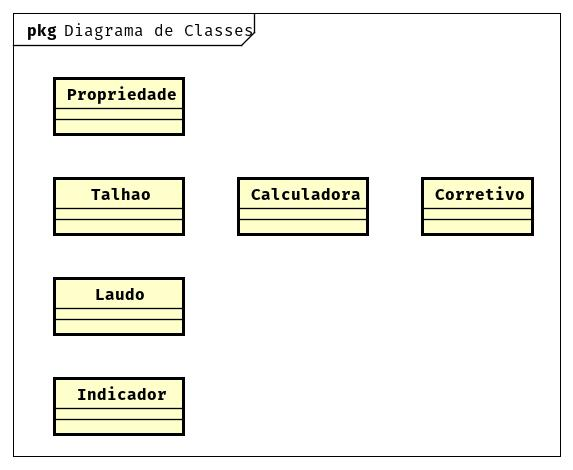
\includegraphics[width=13cm]{./dados/analise/diagramaclasse.jpg}
    \caption{Diagrama de Classes}
    \label{fig:diagramaClasse}
\end{figure}
\clearpage

\section{Projeto de Banco de Dados}
\label{sec:titSecBancoDados}

Segundo \cite{silberschatz2006sistema}, o objetivo do projeto de Banco de Dados é a construção de um conjunto de estruturas que permitam a representação de um dado de forma não redundante e que esse dado possa ser recuperado de forma simples. Este processo geralmente passa em diferentes níveis de abstração. Primeiramente, inicia-se com o entendimento do problema, para depois seguir por diferentes fases de modelagem, até chegar à implementação. Nesse processo, um modelo considerado padrão para a etapa inicial de modelagem é o entidade-relacionamento (ER) \cite{heuser2009projeto}.

\subsection{Diagrama de Entidade-Relacionamento}
\label{sec:titSecDiagER}

A modelagem entidade-relacionamento é a mais utilizada e difundida técnica de modelagem de dados. Nesta técnica, o modelo de dados é representado por meio de um modelo entidade-relacionamento (modelo ER). Comumente, o modelo ER é representado graficamente por meio de um diagrama entidade-relacionamento (DER) \cite{heuser2009projeto}.

A \autoref{fig:diagramaer} representa o DER do projetado neste documento.

\begin{figure}[H]
    \centering
    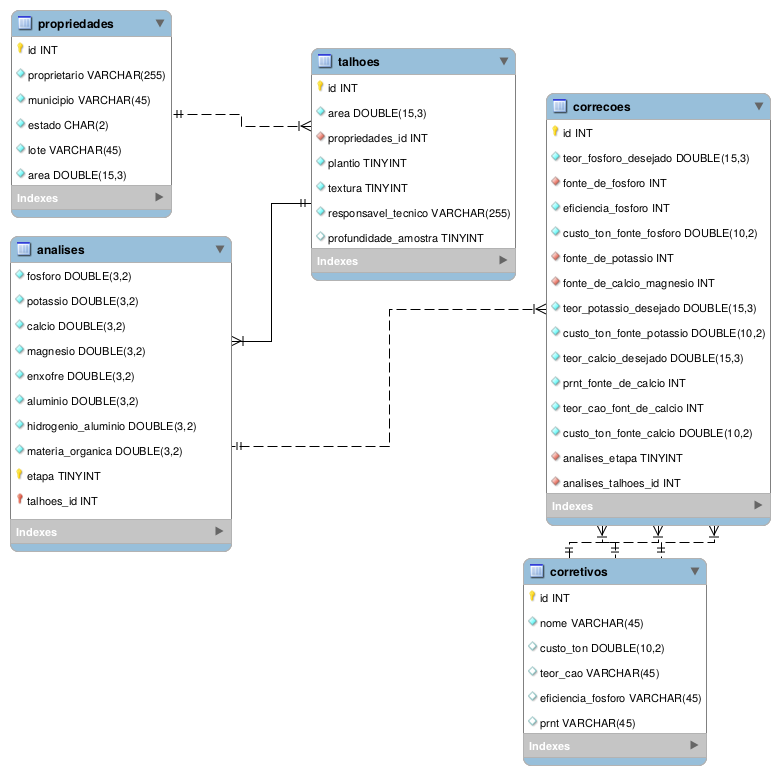
\includegraphics[width=13cm]{./dados/analise/diagramaer.png}
    \caption{Diagrama Entidade-Relacionamento}
    \label{fig:diagramaer}
\end{figure}

\subsection{Dicionário de Dados}
\label{sec:titSecDiagERDicionario}

\begin{landscape}
    \subsubsection{Tabela de Propriedades}
    \label{sec:titSubSecPropriedades}

    \begin{table}[H]
        \centering
        \caption[Tabela \textbf{propriedades}]{Na tabela propriedades ficarão armazenados os dados referentes à propriedade.
            \label{tab:tabela-er-propriedades}}
        \begin{tabular}{|p{4cm}|p{3cm}|p{2cm}|p{1cm}|p{2cm}|p{8cm}|}
            \hline
            Atributo     & Classe       & Domínio  & Bytes & Restrição & Descrição            \\\hline
            id           & Determinante & Numérico & 4     & PK, AI    &                      \\\hline
            proprietario & Simples      & Texto    & 255   & NN        & Nome do proprietário \\\hline
            municipio    & Simples      & Texto    & 255   & NN        & e.g. Dois Vizinhos   \\\hline
            estado       & Simples      & Texto    & 2     & NN        & e.g. PR              \\\hline
            lote         & Simples      & Texto    & 20    & NN        & e.g Q-103            \\\hline
            area         & Simples      & Numérico & 255   & NN        & Em metros quadrados  \\\hline
        \end{tabular}
    \end{table}

    \subsubsection{Tabela de Talhões}
    \label{sec:titSubSecTalhoes}

    \begin{table}[H]
        \centering
        \caption[Tabela \textbf{talhões}]{Na tabela talhões serão armazenados os dados referentes aos talhões da propriedade.
            \label{tab:tabela-er-talhoes}}
        \begin{tabular}{|p{4cm}|p{3cm}|p{2cm}|p{1cm}|p{2cm}|p{8cm}|}
            \hline
            Atributo              & Classe       & Domínio    & Bytes & Restrição & Descrição                        \\\hline
            id                    & Determinante & Numérico   & 4     & PK, AI    &                                  \\\hline
            area                  & Simples      & Numérico   & 10    & NN        & Em metros quadrados              \\\hline
            propriedades\_id      & Composto     & Numérico   & 255   & FK, NN    & Referência à tabela propriedades \\\hline
            plantio               & Simples      & Enumeravel & 1     & NN        & e.g. 1 (Plantio Direto)          \\\hline
            textura               & Simples      & Enumeravel & 1     & NN        & e.g. 2 (Textura Média)           \\\hline
            responsavel\_tecnico  & Simples      & Texto      & 255   & NN        & e.g. Pedro Cecere Filho          \\\hline
            profundidade\_amostra & Simples      & Numérico   & 255   &           & Em centímetros                   \\\hline
        \end{tabular}
    \end{table}

    \subsubsection{Tabela de Análises}
    \label{sec:titSubSecAnalises}

    \begin{table}[H]
        \centering
        \caption[Tabela \textbf{análises}]{Na tabela análises serão armazenados os dados do laudo técnico referente ao talhão.
            \label{tab:tabela-er-analises}}
        \begin{tabular}{|p{4cm}|p{3cm}|p{2cm}|p{1cm}|p{2cm}|p{8cm}|}
            \hline
            Atributo             & Classe       & Domínio  & Bytes & Restrição & Descrição                          \\\hline
            fosforo              & Simples      & Numérico & 4     & NN        & centimol de carga/decimetro cúbico \\\hline
            potassio             & Simples      & Numérico & 4     & NN        & centimol de carga/decimetro cúbico \\\hline
            calcio               & Simples      & Numérico & 4     & NN        & centimol de carga/decimetro cúbico \\\hline
            magnesio             & Simples      & Numérico & 4     & NN        & centimol de carga/decimetro cúbico \\\hline
            enxofre              & Simples      & Numérico & 4     & NN        & centimol de carga/decimetro cúbico \\\hline
            aluminio             & Simples      & Numérico & 4     & NN        & centimol de carga/decimetro cúbico \\\hline
            hidrogenio\_aluminio & Simples      & Numérico & 4     & NN        & centimol de carga/decimetro cúbico \\\hline
            materia\_organica    & Simples      & Numérico & 4     & NN        & centimol de carga/decimetro cúbico \\\hline
            etapa                & Determinante & Numérico & 4     & PK, AI    &                                    \\\hline
            talhoes\_id          & Composto     & Numérico & 4     & PK, FK    & Referência à tabela talhoes        \\\hline
        \end{tabular}
    \end{table}

    \subsubsection{Tabela de Correções}
    \label{sec:titSubSecAnalises}

    \begin{table}[H]
        \centering
        \caption[Tabela \textbf{Correções}]{Na tabela Correções serão armazenados os dados úteis para o cálculo do equilíbrio e correção do solo.
            \label{tab:tabela-er-correcoes}}
        \begin{tabular}{|p{4cm}|p{3cm}|p{2cm}|p{1cm}|p{2cm}|p{8cm}|}
            \hline
            Atributo                    & Classe       & Domínio  & Bytes & Restrição & Descrição                         \\\hline
            id                          & Determinante & Numérico & 4     & PK, AI    &                                   \\\hline
            teor\_fosforo\_desejado     & Simples      & Numérico & 1     & NN        & em percentual                     \\\hline
            fonte\_de\_fosforo          & Composto     & Numérico & 4     & NN        & em referência à tabela corretivos \\\hline
            eficiencia\_fosforo         & Simples      & Numérico & 1     & NN        & em percentual                     \\\hline
            custo\_ton\_fonte\_fosforo  & Simples      & Numérico & 8     & NN        & em R\$/tonelada                   \\\hline
            fonte\_de\_potassio         & Composto     & Numérico & 4     & NN        & em referência à tabela corretivos \\\hline
            fonte\_de\_calcio\_magnesio & Composto     & Numérico & 4     & NN        & em referência à tabela corretivos \\\hline
            teor\_potassio\_desejado    & Simples      & Numérico & 1     & NN        & em percentual                     \\\hline
            custo\_ton\_fonte\_potassio & Simples      & Numérico & 8     & NN        & em R\$/tonelada                   \\\hline
            teor\_calcio\_desejado      & Simples      & Numérico & 1     & NN        & em percentual                     \\\hline
            prnt\_fonte\_de\_calcio     & Simples      & Numérico & 1     & NN        & em percentual                     \\\hline
            teor\_cao\_font\_de\_calcio & Simples      & Numérico & 1     & NN        & em percentual                     \\\hline
            custo\_ton\_fonte\_calcio   & Simples      & Numérico & 8     & NN        & em R\$/tonelada                   \\\hline
            analises\_etapa             & Composto     & Numérico & 4     & FK        & Referência à tabela talhoes       \\\hline
            analises\_talhoes\_id       & Composto     & Numérico & 4     & FK        & Referência à tabela talhoes       \\\hline
        \end{tabular}
    \end{table}

    \subsubsection{Tabela de Correções}
    \label{sec:titSubSecAnalises}

    \begin{table}[H]
        \centering
        \caption[Tabela \textbf{Corretivos}]{Na tabela Corretivos serão armazenados os dados padrões acerca dos corretivos.
            \label{tab:tabela-er-correcoes}}
        \begin{tabular}{|p{4cm}|p{3cm}|p{2cm}|p{1cm}|p{2cm}|p{8cm}|}
            \hline
            Atributo            & Classe       & Domínio  & Bytes & Restrição & Descrição       \\\hline
            id                  & Determinante & Numérico & 4     & PK, AI    &                 \\\hline
            nome                & Simples      & Texto    & 255   & NN        & em percentual   \\\hline
            custo\_ton          & Simples      & Numérico & 8     &           & em R\$/tonelada \\\hline
            teor\_cao           & Simples      & Numérico & 1     &           & em percentual   \\\hline
            eficiencia\_fosforo & Simples      & Numérico & 1     &           & em percentual   \\\hline
            prnt                & Simples      & Numérico & 1     &           & em percentual   \\\hline
        \end{tabular}
    \end{table}

\end{landscape}
\clearpage

\subsection{Diagrama de Implantação}
\label{sec:titSecDiagDeploy}

O Diagrama de Implantação determina as necessidades de \textit{hardware} do sistema, as características físicas como servidores, estações, topologias e protocolos de comunicação \cite{guedes2018uml}, destacando todos as necessidades físicas no qual o sistema deverá ser executado. Também é mostrado como será a distribuição dos módulos do sistema nos momentos onde a aplicação estará sendo executada em diferentes servidores.

\begin{figure}[H]
    \centering
    \caption{Representação do Diagrama de Implantação}
    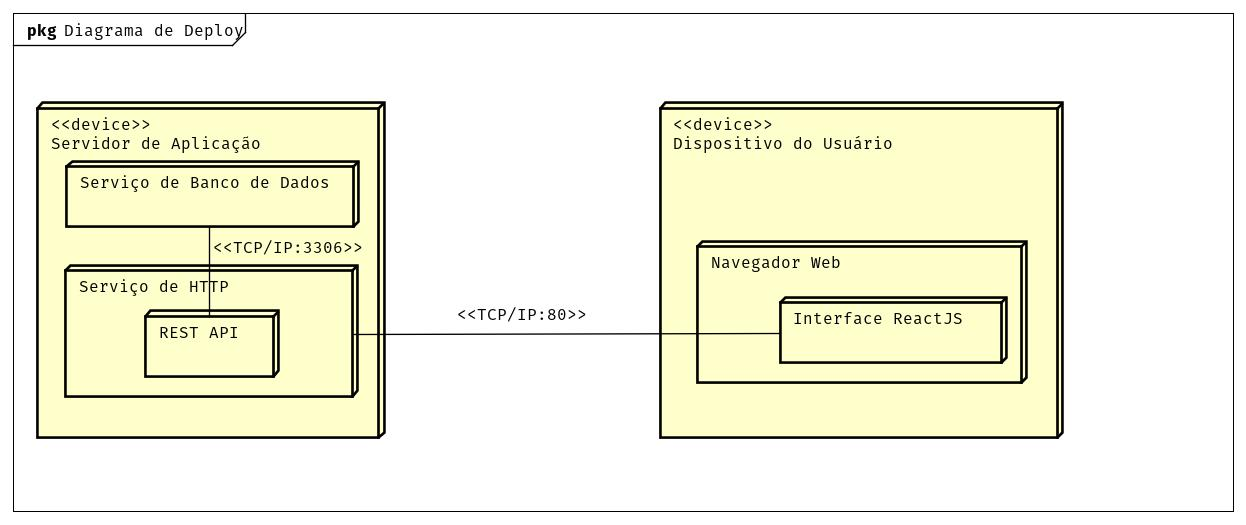
\includegraphics[width=13cm]{dados/figuras/diagramadeploy.jpg}
    \label{fig:diagramaDeploy}
    \fonte{Autoria própria}
\end{figure}

A \autoref{fig:diagramaDeploy} mostra a aplicação desse conceito no projeto. Nela é possível observar a distribuição do sistema em dois nós principais. O primeiro é o servidor de aplicação, que faz o encapsulamento do servidor Apache. Nesse mesmo servidor é possível observar a presença de um servidor MySQL, o qual será responsável por armazenar os dados do sistema e só receberá acessos locais.
O outro nó, representa o lado do cliente da aplicação, responsável pelas chamadas ao recursos contidos no servidor \textit{web} por meio de requisições Ajax, por meio do protocolo HTTP.

\clearpage

\section{PROTÓTIPOS DE TELA}
\label{sec:titSecPrototipos}

% Os protótipos de tela são uma versão inicial de um sistema. Eles são usados, dentre outras razões, para descobrir mais sobre um problema e suas possíveis soluções. O desenvolvimento rápido e iterativo do protótipo previne gastos desnecessários e custos controlados e os \textit{stakeholders} podem fazer usos pontuais de partes do sistema desde o início do desenvolvimento \citeonline{Sommerville10}.

% Além disso, os protótipos podem ajudar na antecipação de mudanças que podem ser requisitadas.
% Para o presente projeto foram desenvolvidas três interfaces para dois tamanhos diferentes de tela, simulando um dispositivo de tela maior (\textit{desktop}, \textit{tablet}) e outro para telas menores (\textit{smartphones}).

% O modelo de prototipação é ideal quando o cliente não tem os requisitos muito bem definidos, que é o caso do aplicativo estudado neste documento. Visto que os requisitos foram levantados com base em uma planilha, conforme explicado anteriormente na \autoref{sub:processo}.

Nas próximas subseções serão exibidos os protótipos de tela para três principais operações que o usuário poderá realizar no sistema, que são a tela que o usuário é enviado após fazer o \textit{login}, a tela para criação de um novo recurso no sistema e a tela de exibição de um recurso.

\subsection{Protótipos para tela inicial do sistema}
\label{sec:titSecPrototiposHome}

As Figuras \ref{fig:prototipo_home_desk} e \ref{fig:prototipo_home_mobile}, representam a visão da página inicial do sistema, que será exibida após o login do usuário. É possível observar que logo na parte superior, existirão quadros informativos sobre a quantidade de propriedades assistidas, quantidade de cidades atendidas e a área em hectares que foram tratadas (ou corrigidas). Logo abaixo serão exibidas as últimas correções realizadas pelo usuário.

\begin{figure}[H]
    \centering
    \caption{Página que será exibida após o login do usuário na visão de um dispositivo \textit{desktop}}
    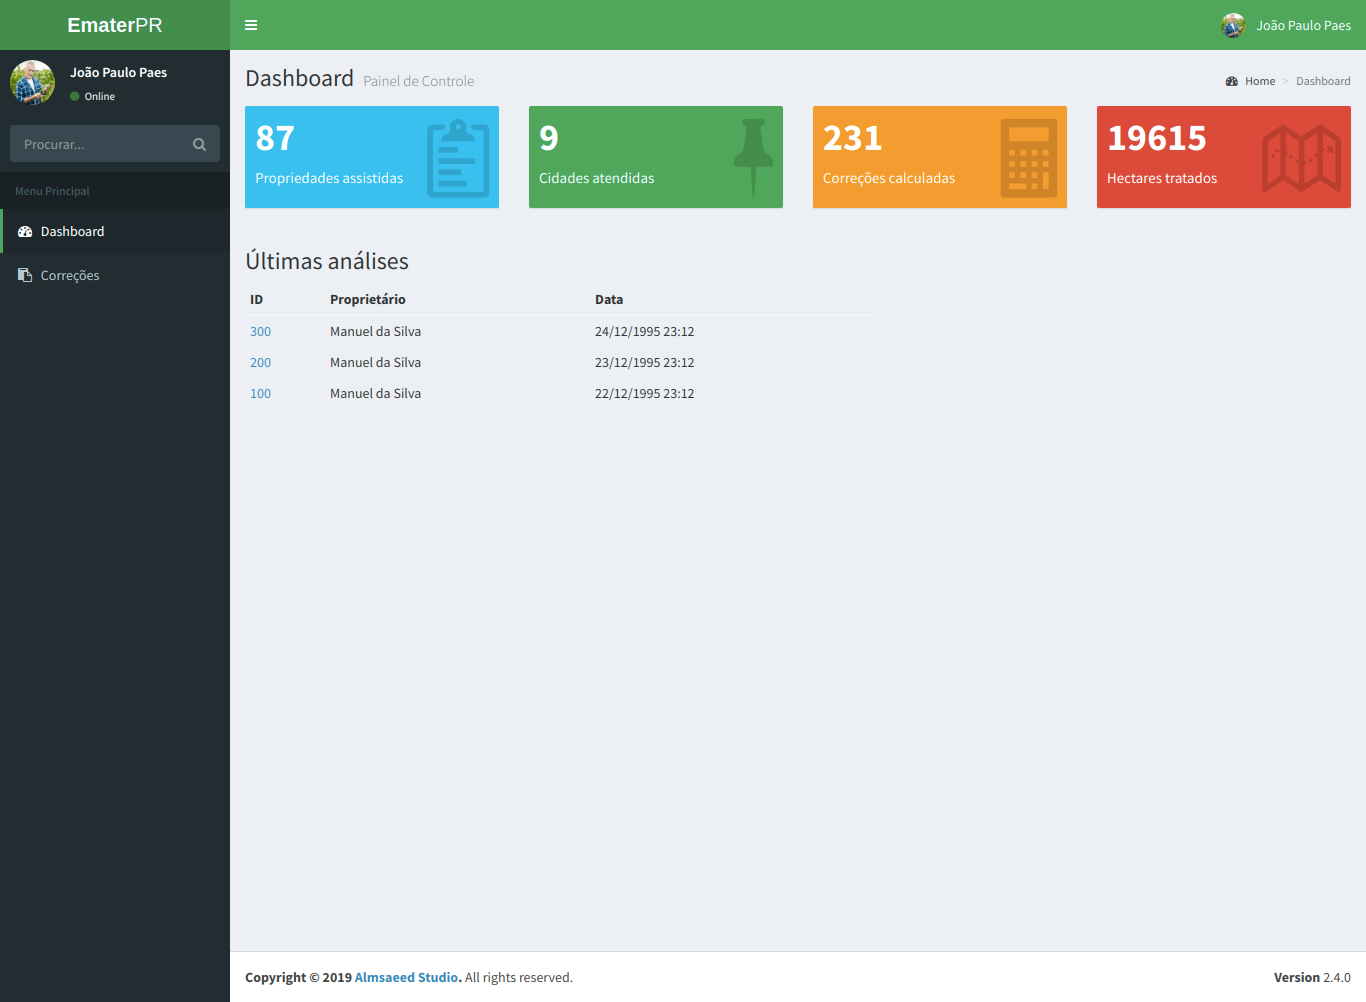
\includegraphics[width=13cm]{./dados/figuras/prototipos/home_desktop.png}
    \label{fig:prototipo_home_desk}
    \fonte{Autoria própria}
\end{figure}

\begin{figure}[H]
    \centering
    \caption{Página que será exibida após o login do usuário na visão de um dispositivo \textit{mobile}}
    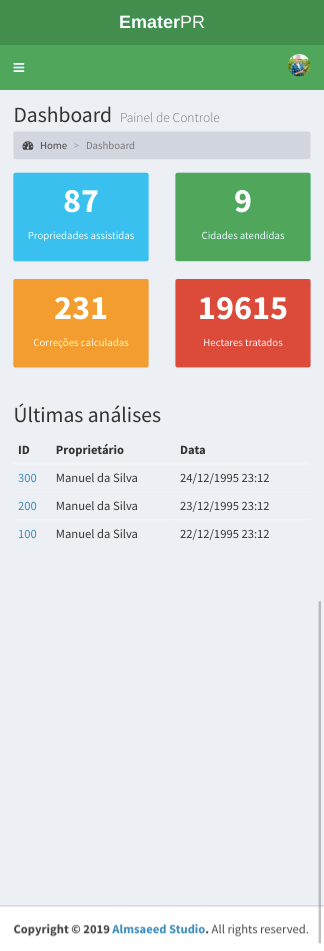
\includegraphics[width=6cm]{./dados/figuras/prototipos/home_mobile.png}
    \label{fig:prototipo_home_mobile}
    \fonte{Autoria própria}
\end{figure}

\subsection{Protótipos para tela de cadastro de informação}
\label{sec:titSecPrototiposCreate}

A tela de cadastro de informações foi pensada para ser intuitiva e reativa como a planilha. Como é um formulário grande, será divido em \textit{steps} que serão exibidos na parte superior do formulário, tendo a descrição do que deve ser feito naquele \textit{step} logo abaixo. Já o formulário propriamente dito terá uma interface reativa, que lembra a planilha.

No exemplo mostrado nas Figuras \ref{fig:prototipo_create_desk} e \ref{fig:prototipo_create_mobile}, é possível observar que caso o valor de um campo esteja no intervalo ideal, este deverá ter a sua \textit{label} e o contorno destacados em verde. Enquanto se o valor estiver fora do intervalo, em âmbar. 

\begin{figure}[H]
    \centering
    \caption{Criação de recurso na visão de um dispositivo \textit{desktop}}
    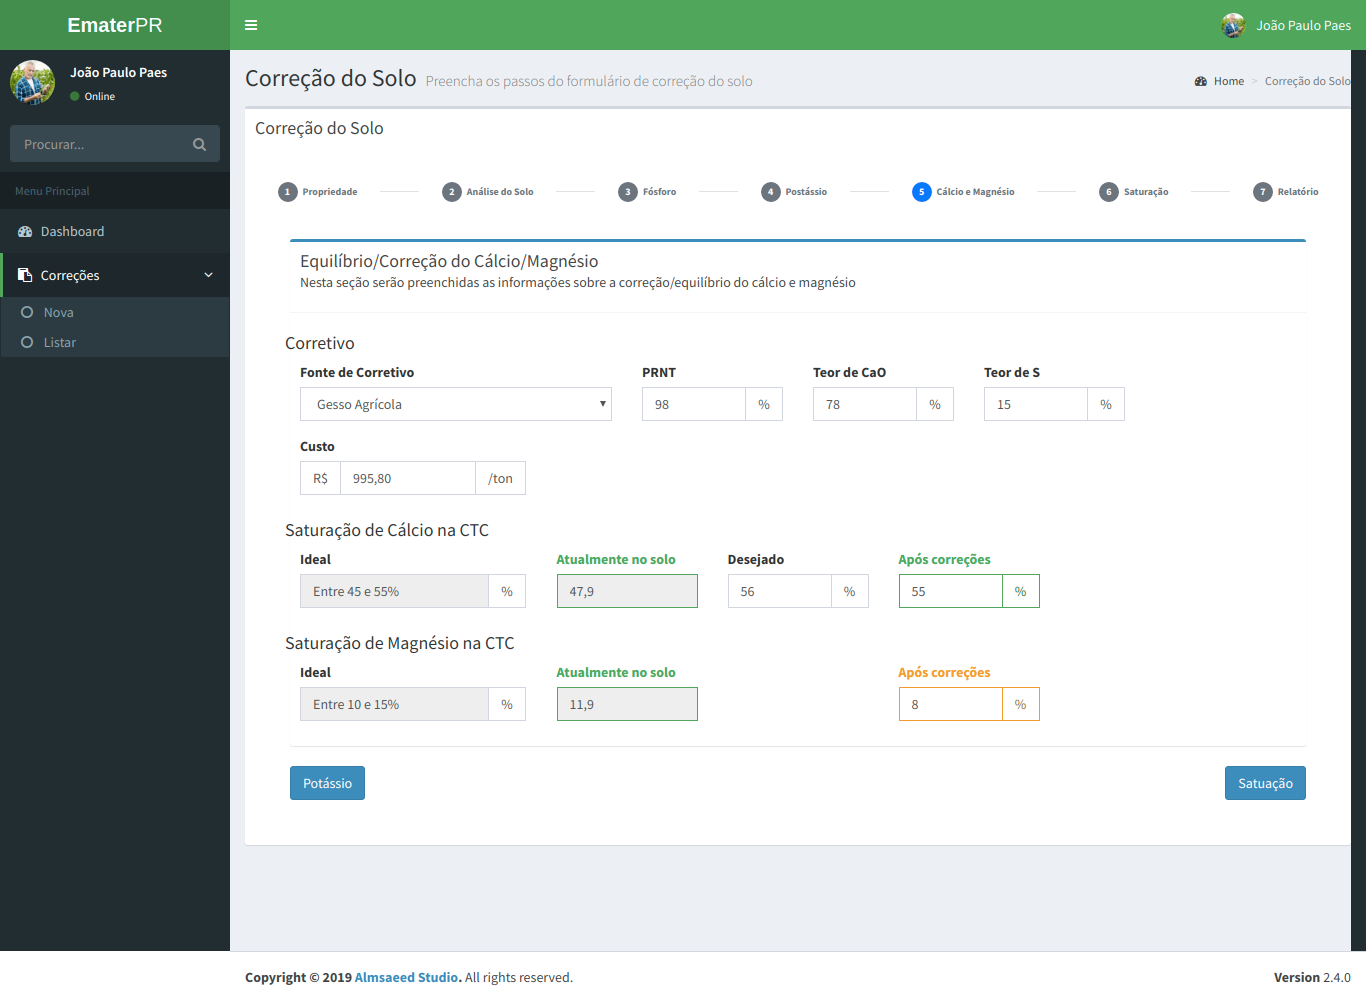
\includegraphics[width=13cm]{./dados/figuras/prototipos/create_desktop.png}
    \label{fig:prototipo_create_desk}
    \fonte{Autoria própria}
\end{figure}

\begin{figure}[H]
    \centering
    \caption{Criação de recurso na visão de um dispositivo \textit{mobile}}
    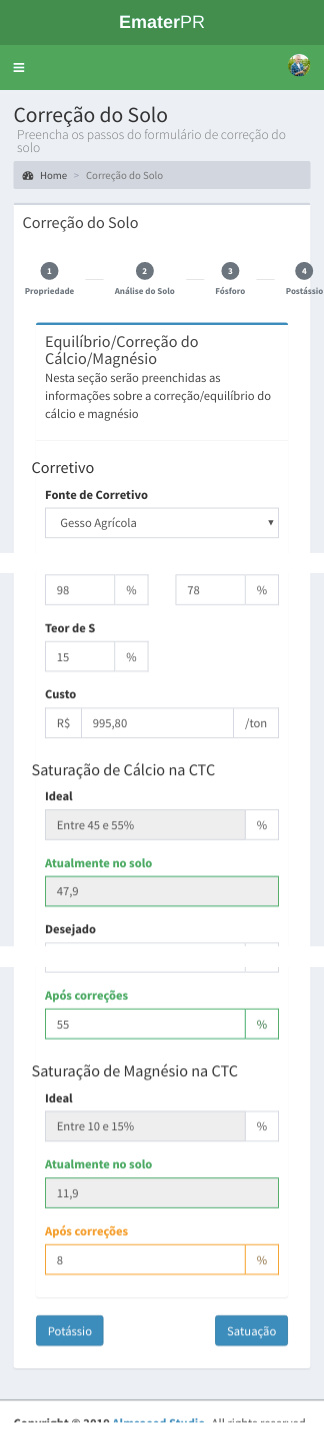
\includegraphics[width=6cm]{./dados/figuras/prototipos/create_mobile.png}
    \label{fig:prototipo_create_mobile}
    \fonte{Autoria própria}
\end{figure}


\subsection{Protótipos para tela de exibição de informação}
\label{sec:titSecPrototiposShow}

A tela de exibição da informação também seguirá o modelo de \textit{steps}. Ela deverá ser dividia em 3 colunas para representar os três estados da correção do solo: naquele momento, desejado e após as correções. É possível notar que os textos deverão estar coloridos de acordo com o caso no qual se encaixa. Acima do valor, amarelo. Abaixo do valor, vermelho. No intervalo, verde.

\begin{figure}[H]
    \centering
    \caption{Visualização de recurso na visão de um dispositivo \textit{desktop}}
    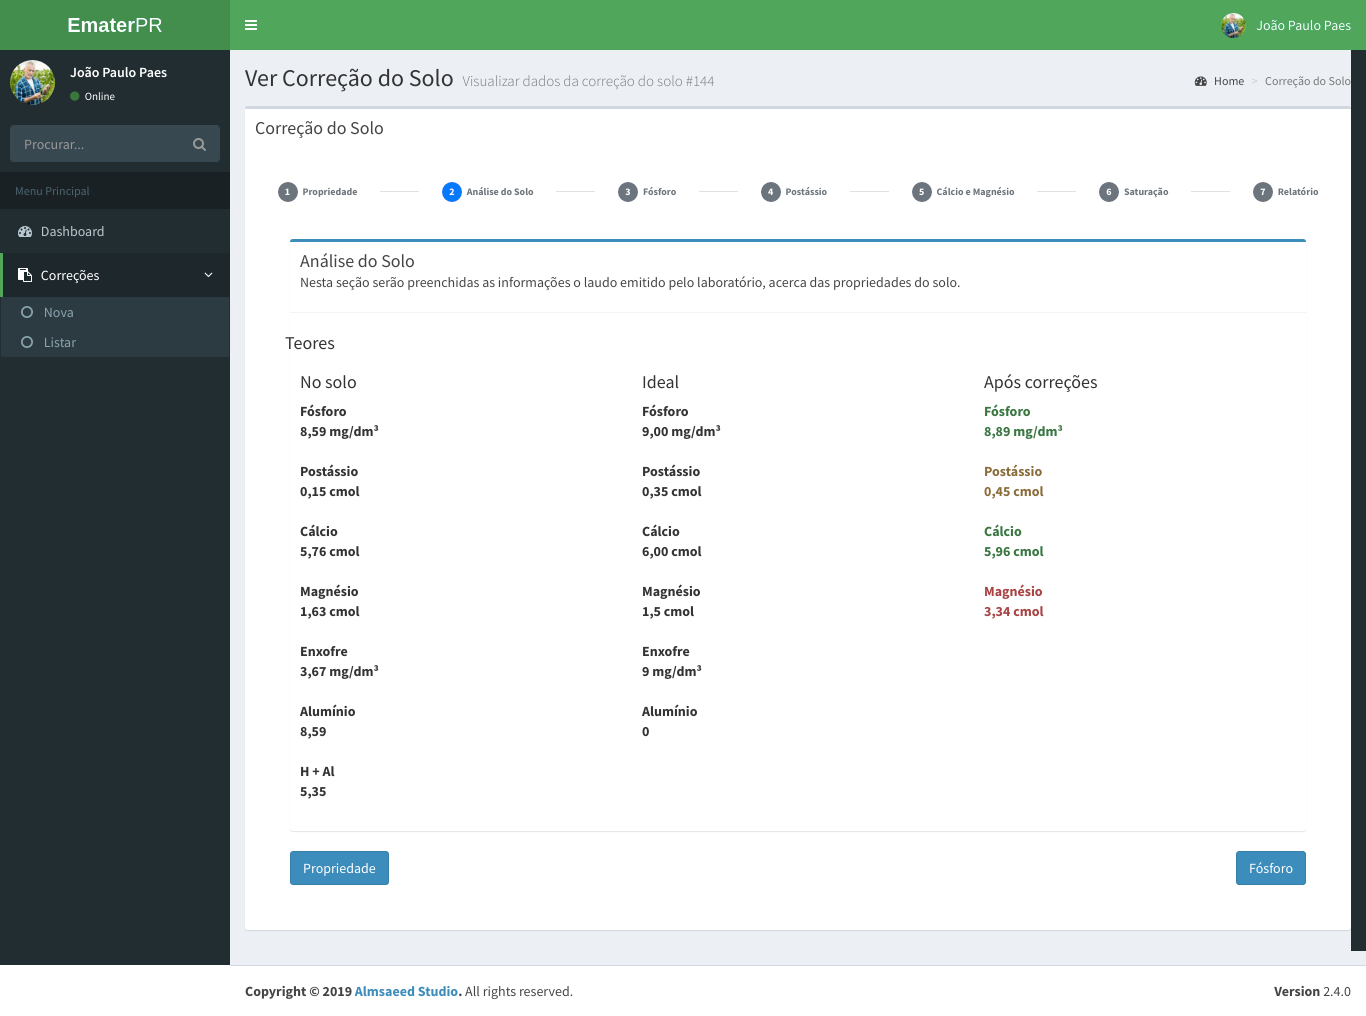
\includegraphics[width=13cm]{./dados/figuras/prototipos/show_desktop.png}
    \label{fig:prototipo_show_desk}
    \fonte{Autoria própria}
\end{figure}

\begin{figure}[H]
    \centering
    \caption{Visualização de recurso na visão de um dispositivo \textit{mobile}}
    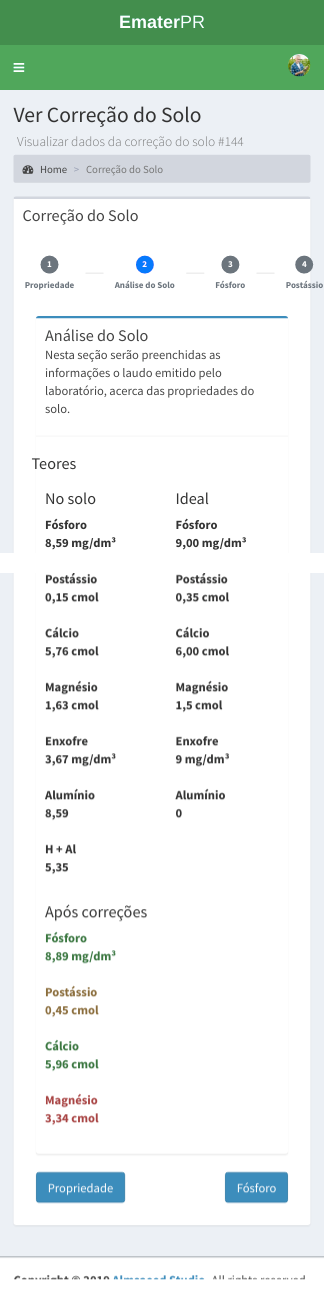
\includegraphics[width=6cm]{./dados/figuras/prototipos/show_mobile.png}
    \label{fig:prototipo_show_mobile}
    \fonte{Autoria própria}
\end{figure}
\clearpage                   % Análise
% RESULTADOS-------------------------------------------------------------------

\chapter{ANÁLISE E DISCUSSÃO DOS RESULTADOS}

Cada capítulo deve conter uma pequena introdução (tipicamente, um ou dois parágrafos) que deve deixar claro o objetivo e o que será discutido no capítulo, bem como a organização do capítulo.
                    % Resultados
% ORIENTAÇÕES GERAIS------------------------------------------------------------


% SOBRE AS ILUSTRAÇÕES----------------------------------------------------------
\chapter{SOBRE AS ILUSTRAÇÕES}
\label{chap:apSobreIlust}

A seguir exemplifica-se como inserir ilustrações no corpo do trabalho. As ilustrações serão indexadas automaticamente em suas respectivas listas. A numeração sequencial de figuras, tabelas e equações também ocorre de modo automático.

Referências cruzadas são obtidas através dos comandos \verb|\label{}| e \verb|\ref{}|. Sendo assim, não é necessário por exemplo, saber que o número de certo capítulo é \ref{chap:fundamentacaoTeorica} para colocar o seu número no texto. Outra forma que pode ser utilizada é esta: \autoref{chap:fundamentacaoTeorica}, facilitando a inserção, remoção e manejo de elementos numerados no texto sem a necessidade de renumerar todos esses elementos.

% FIGURAS-----------------------------------------------------------------------
\chapter{FIGURAS}
\label{chap:figuras}

Exemplo de como inserir uma figura. A \autoref{fig:figura-exemplo1} aparece automaticamente na lista de figuras. Para saber mais sobre o uso de imagens no \LaTeX{} consulte literatura especializada \cite{Goossens2007}.

Os arquivos das figuras devem ser armazenados no diretório de "/dados".

\begin{figure}[!htb]
    \centering
    \caption{Exemplo de Figura}
    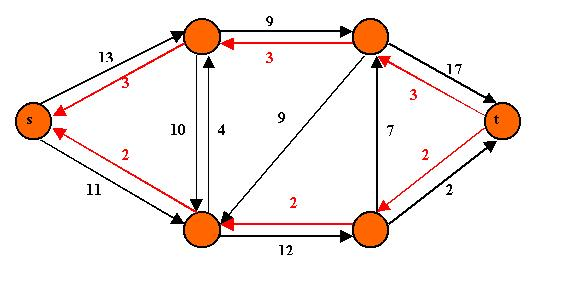
\includegraphics[width=0.5\textwidth]{./dados/figuras/figura1}
    \fonte{\citeonline{IRL2014}}
    \label{fig:figura-exemplo1}
\end{figure}

% QUADROS E TABELAS---------------------------------------------------------------
\chapter{QUADROS E TABELAS}
\label{chap:tabelas}

Exemplo de como inserir o \autoref{qua:quadro-exemplo1} e a \autoref{tab:tabela-exemplo1}. Ambos aparecem automaticamente nas suas respectivas listas. Para saber mais informações sobre a construção de tabelas no \LaTeX{} consulte literatura especializada \cite{Mittelbach2004}.

Ambos os elementos (Quadros e Tabelas) devem ser criados em arquivos separados para facilitar manutenção e armazenados no diretório de "/dados".

\begin{quadro}[!htb]
    \centering
    \caption{Exemplo de Quadro.\label{qua:quadro-exemplo1}}
    \begin{tabular}{|p{7cm}|p{7cm}|}
        \hline
        \textbf{BD Relacionais} & \textbf{BD Orientados a Objetos} \\
        \hline
        Os dados são passivos, ou seja, certas operações limitadas podem ser automaticamente acionadas quando os dados são usados. Os dados são ativos, ou seja, as solicitações fazem com que os objetos executem seus métodos. & Os processos que usam dados mudam constantemente. \\
        \hline
    \end{tabular}
    \fonte{\citeonline{Barbosa2004}}
\end{quadro}


A diferença entre quadro e tabela está no fato que um quadro é formado por linhas horizontais e verticais. Deve ser utilizado quando o conteúdo é majoritariamente não-numérico. O número do quadro e o título vem acima do quadro, e a fonte, deve vir abaixo. E Uma tabela é formada apenas por linhas verticais. Deve ser utilizada quando o conteúdo é majoritariamente numérico. O número da tabela e o título vem acima da tabela, e a fonte, deve vir abaixo, tal como no quadro.

\begin{table}[!htb]
    \centering
    \caption[Resultado dos testes]{Resultado dos testes.
    \label{tab:tabela-exemplo1}}
    \begin{tabular}{rrrrr}
        \toprule
            & Valores 1 & Valores 2 & Valores 3 & Valores 4 \\
        \midrule
            Caso 1 & 0,86 & 0,77 & 0,81 & 163 \\
            Caso 2 & 0,19 & 0,74 & 0,25 & 180 \\
            Caso 3 & 1,00 & 1,00 & 1,00 & 170 \\
        \bottomrule
    \end{tabular}
    \fonte{\citeonline{Barbosa2004}}
\end{table}


% EQUAÇÕES-----------------------------------------------------------------------
\chapter{EQUAÇÕES}
\label{chap:equacoes}

Exemplo de como inserir a \autoref{eq:equacao-exemplo1} e a Eq. \ref{eq:equacao-exemplo2} no corpo do texto \footnote{Deve-se atentar ao fato de a formatação das equações ficar muito boa esteticamente.}. Observe que foram utilizadas duas formas distintas para referenciar as equações.

\begin{equation}
    X(s) = \int\limits_{t = -\infty}^{\infty} x(t) \, \text{e}^{-st} \, dt
    \label{eq:equacao-exemplo1}
\end{equation}

\begin{equation}
    F(u, v) = \sum_{m = 0}^{M - 1} \sum_{n = 0}^{N - 1} f(m, n) \exp \left[ -j 2 \pi \left( \frac{u m}{M} + \frac{v n}{N} \right) \right]
    \label{eq:equacao-exemplo2}
\end{equation}

% ALGORITMOS-----------------------------------------------------------------------
\chapter{ALGORITMOS}
\label{chap:algoritmos}

Exemplo de como inserir um algoritmo. Para inserção de algoritmos utiliza-se o pacote {\ttfamily algorithm2e} que já está devidamente configurado dentro do template.

Os algoritmos devem ser criados em arquivos separados para facilitar manutenção e armazenados no diretório de "/dados".\\
\\

\begin{algorithm}
    \caption{Exemplo de Algoritmo}
    \KwIn{o número $n$ de vértices a remover, grafo original $G(V, E)$}
    \KwOut{grafo reduzido $G'(V,E)$}
    $removidos \leftarrow 0$ \\
    \While {removidos $<$ n } {
        $v \leftarrow$ Random$(1, ..., k) \in V$ \\
            \For {$u \in adjacentes(v)$} {
                remove aresta (u, v)\\
                $removidos \leftarrow removidos + 1$\\
            }
            \If {há  componentes desconectados} {
                remove os componentes desconectados\\
            }
        }
\end{algorithm}


% SOBRE AS LISTAS--------------------------------------------------------------------
\chapter{SOBRE AS LISTAS}
\label{chap:apSobreLista}

Para construir listas de "\textit{bullets}"{} ou listas enumeradas, inclusive listas aninhadas, é utilizado o pacote \verb|paralist|.

Exemplo de duas listas não numeradas aninhadas, utilizando o comando \verb|\itemize|. Observe a indentação, bem como a mudança automática do tipo de "\textit{bullet}"{} nas listas aninhadas.

\begin{itemize}
    \item item não numerado 1
    \item item não numerado 2
    \begin{itemize}
        \item subitem não numerado 1
        \item subitem não numerado 2
        \item subitem não numerado 3
    \end{itemize}
    \item item não numerado 3
\end{itemize}

Exemplo de duas listas numeradas aninhadas, utilizando o comando \verb|\enumerate|. Observe a numeração progressiva e indentação das listas aninhadas.

\begin{enumerate}
    \item item numerado 1
    \item item numerado 2
    \begin{enumerate}
        \item subitem numerado 1
        \item subitem numerado 2
        \item subitem numerado 3
    \end{enumerate}
    \item item numerado 3
\end{enumerate}

% SOBRE AS CITAÇÕES E CHAMADAS DE REFERÊNCAS----------------------------------------------
\chapter{SOBRE AS CITAÇÕES E CHAMADAS DE REFERÊNCAS}
\label{chap:apSobreCita}

Citações são trechos de texto ou informações obtidas de materiais consultadss quando da elaboração do trabalho. São utilizadas no texto com o propósito de esclarecer, completar e embasar as ideias do autor. Todas as publicações consultadas e utilizadas (por meio de citações) devem ser listadas, obrigatoriamente, nas referências bibliográficas, para preservar os direitos autorais. São classificadas em citações indiretas e diretas.

% CITAÇÕES INDIRETAS-----------------------------------------------------------------------
\chapter{CITAÇÕES INDIRETAS}
\label{chap:citacoesLivres}

É a transcrição, com suas próprias palavras, das idéias de um autor, mantendo-se o sentido original. A citação indireta é a maneira que o pesquisador tem de ler, compreender e gerar conhecimento a partir do conhecimento de outros autores. Quanto à chamada da referência, ela pode ser feita de duas maneiras distintas, conforme o nome do(s) autor(es) façam parte do seu texto ou não. Exemplo de chamada fazendo parte do texto:\\
\\Enquanto \citeonline{Maturana2003} defendem uma epistemologia baseada na biologia. Para os autores, é necessário rever \ldots.\\

A chamada de referência foi feita com o comando \verb|\citeonline{chave}|, que produzirá a formatação correta.

A segunda forma de fazer uma chamada de referência deve ser utilizada quando se quer evitar uma interrupção na sequência do texto, o que poderia, eventualmente, prejudicar a leitura. Assim, a citação é feita e imediatamente após a obra referenciada deve ser colocada entre parênteses. Porém, neste caso específico, o nome do autor deve vir em caixa alta, seguido do ano da publicação. Exemplo de chamada não fazendo parte do texto:\\
\\Há defensores da epistemologia baseada na biologia que argumentam em favor da necessidade de \ldots \cite{Maturana2003}.\\

Nesse caso a chamada de referência deve ser feita com o comando \verb|\cite{chave}|, que produzirá a formatação correta.

% CITAÇÕES DIRETAS-----------------------------------------------------------------------
\chapter{CITAÇÕES DIRETAS}
\label{chap:citacoesLiterais}

É a transcrição ou cópia de um parágrafo, de uma frase, de parte dela ou de uma expressão, usando exatamente as mesmas palavras adotadas pelo autor do trabalho consultado.

Quanto à chamada da referência, ela pode ser feita de qualquer das duas maneiras já mencionadas nas citações indiretas, conforme o nome do(s) autor(es) façam parte do texto ou não. Há duas maneiras distintas de se fazer uma citação direta, conforme o trecho citado seja longo ou curto.

Quando o trecho citado é longo (4 ou mais linhas) deve-se usar um parágrafo específico para a citação, na forma de um texto recuado (4 cm da margem esquerda), com tamanho de letra menor e espaçamento entrelinhas simples. Exemplo de citação longa:
\\\begin{citacao}
    Desse modo, opera-se uma ruptura decisiva entre a reflexividade filosófica, isto é a possibilidade do sujeito de pensar e de refletir, e a objetividade científica. Encontramo-nos num ponto em que o conhecimento científico está sem consciência. Sem consciência moral, sem consciência reflexiva e também subjetiva. Cada vez mais o desenvolvimento extraordinário do conhecimento científico vai tornar menos praticável a própria possibilidade de reflexão do sujeito sobre a sua pesquisa \cite[p.~28]{Silva2000}.
\end{citacao}

Para fazer a citação longa deve-se utilizar os seguintes comandos:
\begin{verbatim}
\begin{citacao}
<texto da citacao>
\end{citacao}
\end{verbatim}

No exemplo acima, para a chamada da referência o comando \verb|\cite[p.~28]{Silva2000}| foi utilizado, visto que os nomes dos autores não são parte do trecho citado. É necessário também indicar o número da página da obra citada que contém o trecho citado.

Quando o trecho citado é curto (3 ou menos linhas) ele deve inserido diretamente no texto entre aspas. Exemplos de citação curta:\\
\\A epistemologia baseada na biologia parte do princípio de que "assumo que não posso fazer referência a entidades independentes de mim para construir meu explicar" \cite[p.~35]{Maturana2003}.\\
\\A epistemologia baseada na biologia de \citeonline[p.~35]{Maturana2003} parte do princípio de que "assumo que não posso fazer referência a entidades independentes de mim para construir meu explicar".

% DETALHES SOBRE AS CHAMADAS DE REFERÊNCIAS---------------------------------------------------------
\chapter{DETALHES SOBRE AS CHAMADAS DE REFERÊNCIAS}
\label{chap:referUtilizadas}

Outros exemplos de comandos para as chamadas de referências e o resultado produzido por estes:\\
\\\citeonline{Maturana2003} \ \ \  \verb|\citeonline{Maturana2003}|\\
\citeonline{Barbosa2004} \ \ \   \verb|\citeonline{Barbosa2004}|\\
\cite[p.~28]{Silva2000} \ \ \  \verb|\cite[p.~28]{Silva2000}|\\
\citeonline[p.~33]{Silva2000} \ \ \   \verb|\citeonline[p.~33]{v}|\\
\cite[p.~35]{Maturana2003} \ \ \   \verb|\cite[p.~35]{Maturana2003}|\\
\citeonline[p.~35]{Maturana2003} \ \ \   \verb|\citeonline[p.~35]{Maturana2003}|\\
\cite{Barbosa2004,Maturana2003} \ \ \   \verb|\cite{Barbosa2004,Maturana2003}|\\

% SOBRE AS REFERÊNCIAS BIBLIOGRÁFICAS-------------------------------------------------------
\chapter{SOBRE AS REFERÊNCIAS BIBLIOGRÁFICAS}
\label{chap:apSobreRefer}

A bibliografia é feita no padrão \textsc{Bib}\TeX{}. As referências são colocadas em um arquivo separado. Neste template as referências são armazenadas no arquivo "base-referencias.bib".

Existem diversas categorias documentos e materiais componentes da bibliografia. A classe abn\TeX{} define as seguintes categorias (entradas):

\begin{verbatim}
@book
@inbook
@article
@phdthesis
@mastersthesis
@monography
@techreport
@manual
@proceedings
@inproceedings
@journalpart
@booklet
@patent
@unpublished
@misc
\end{verbatim}

Cada categoria (entrada) é formatada pelo pacote \citeonline{abnTeX22014d} de uma forma específica. Algumas entradas foram introduzidas especificamente para atender à norma \citeonline{NBR6023:2002}, são elas: \verb|@monography|, \verb|@journalpart|,\verb|@patent|. As demais entradas são padrão \textsc{Bib}\TeX{}. Para maiores detalhes, refira-se a \citeonline{abnTeX22014d}, \citeonline{abnTeX22014b}, \citeonline{abnTeX22014c}.

% NOTAS DE RODAPÉ--------------------------------------------------------------------------
\chapter{NOTAS DE RODAPÉ}
\label{chap:notasRodape}

As notas de rodapé pode ser classificadas em duas categorias: notas explicativas\footnote{é o tipo mais comum de notas que destacam, explicam e/ou complementam o que foi dito no corpo do texto, como esta nota de rodapé, por exemplo.} e notas de referências. A notas de referências, como o próprio nome ja indica, são utilizadas para colocar referências e/ou chamadas de referências sob certas condições.
                   % Capítulo com Orientações de uso do Template
% CONCLUSÃO--------------------------------------------------------------------

\chapter{CONCLUSÃO}
\label{chap:conclusao}

Parte final do texto, na qual se apresentam as conclusões do trabalho acadêmico. É importante fazer uma análise crítica do trabalho, destacando os principais resultados e as contribuições do trabalho para a área de pesquisa.

\section{TRABALHOS FUTUROS}
\label{sec:trabalhosFuturos}

Também deve indicar, se possível e/ou conveniente, como o trabalho pode ser estendido ou aprimorado.

\section{CONSIDERAÇÕES FINAIS}
\label{sec:consideracoesFinais}

Encerramento do trabalho acadêmico.
                 			   % Conclusão

\postextual
% INSERE ELEMENTOS PÓS-TEXTUAIS
% REFERÊNCIAS------------------------------------------------------------------

% Carrega o arquivo "base-referencias.bib" e extrai automaticamente as referências citadas

\bibliography{./base-referencias}
\bibliographystyle{abntex2-alf} % Define o estilo ABNT para formatar a lista de referências
% OBSERVAÇÕES------------------------------------------------------------------
% Este arquivo não precisa ser alterado.
           			   % Referências
% APÊNDICES--------------------------------------------------------------------

\begin{apendicesenv}
\partapendices

% Primeiro apêndice------------------------------------------------------------
\chapter{Nome do apêndice} % Edite para alterar o título deste apêndice
\label{chap:apendiceA}

Lembre-se que a diferença entre apêndice e anexo diz respeito à autoria do texto e/ou material ali colocado.

Caso o material ou texto suplementar ou complementar seja de sua autoria, então ele deverá ser colocado como um apêndice. Porém, caso a autoria seja de terceiros, então o material ou texto deverá ser colocado como anexo.

Caso seja conveniente, podem ser criados outros apêndices para o seu trabalho acadêmico. Basta recortar e colar este trecho neste mesmo documento. Lembre-se de alterar o "label"{} do apêndice.

Não é aconselhável colocar tudo que é complementar em um único apêndice. Organize os apêndices de modo que, em cada um deles, haja um único tipo de conteúdo. Isso facilita a leitura e compreensão para o leitor do trabalho.

% Novo apêndice----------------------------------------------------------------
\chapter{Nome do outro apêndice}
\label{chap:apendiceB}

conteúdo do novo apêndice

\end{apendicesenv}
             			   % Apêndices
% ANEXO------------------------------------------------------------------------

\begin{anexosenv}
\partanexos

% Primeiro anexo---------------------------------------------------------------
\chapter{Nome do anexo}     % edite para alterar o título deste anexo
\label{chap:anexoA}

Lembre-se que a diferença entre apêndice e anexo diz respeito à autoria do texto e/ou material ali colocado.

Caso o material ou texto suplementar ou complementar seja de sua autoria, então ele deverá ser colocado como um apêndice. Porém, caso a autoria seja de terceiros, então o material ou texto deverá ser colocado como anexo.

Caso seja conveniente, podem ser criados outros anexos para o seu trabalho acadêmico. Basta recortar e colar este trecho neste mesmo documento. Lembre-se de alterar o "label"{} do anexo.

Organize seus anexos de modo a que, em cada um deles, haja um único tipo de conteúdo. Isso facilita a leitura e compreensão para o leitor do trabalho. É para ele que você escreve.

% Novo anexo-------------------------------------------------------------------
\chapter{Nome do outro anexo}
\label{chap:anexoB}

conteúdo do outro anexo

\end{anexosenv}
               			   % Anexos

\end{document}
